\documentclass{article}
\usepackage{titlesec}
%Referencias
\usepackage[style=authortitle,backend=bibtex]{biblatex}
\addbibresource{analysis.bib}

%Paquetes
\usepackage[left=4cm, right=4cm]{geometry}
\usepackage{palatino}%Fuente
\usepackage{graphicx}%Imágenes
\usepackage{float}%Imágenes
\usepackage{subcaption}%Imágenes
\usepackage{enumitem}%Listas
\usepackage{parskip}%Espacio entre párrafos
\usepackage{multicol}
\usepackage{amsthm,thmtools,xcolor}
\usepackage{amssymb}%Mate
\usepackage{amsmath}%Mate
\usepackage{tikz}%Mate (diagramas)
\usepackage{dutchcal}
\usepackage{tikz-cd}
\usepackage{xcolor}
\definecolor{blue-violet}{rgb}{0.54, 0.17, 0.89}
\usetikzlibrary{%
	matrix,%
	calc,%
	arrows,%
	shapes,
	decorations.markings,backgrounds,calc,intersections
}
\usepackage[bookmarks,bookmarksopen,bookmarksdepth=3]{hyperref}%Links a lugares en el texto
\hypersetup{%colores
	colorlinks=true,
	urlcolor=blue,
	linkcolor=magenta,
	citecolor=blue,
	filecolor=blue,
	urlbordercolor=white,
	linkbordercolor=white,
	citebordercolor=white,
	filebordercolor=white
}
\usepackage{cleveref}


%Referencias
%\usepackage[style=authortitle,backend=bibtex]{biblatex}
%\addbibresource{analysis.bib}

\definecolor{blue-violet}{rgb}{0.54, 0.17, 0.89}
\definecolor{azure}{rgb}{0.0, 0.5, 1.0}
\definecolor{green(ncs)}{rgb}{0.0, 0.62, 0.42}
\definecolor{forestgreen}{rgb}{0.13, 0.55, 0.13}
\definecolor{limegreen}{rgb}{0.2, 0.8, 0.2}
\definecolor{palatinateblue}{rgb}{0.15, 0.23, 0.89}
\definecolor{trueblue}{rgb}{0.0, 0.45, 0.81}
\definecolor{goldenyellow}{rgb}{1.0, 0.87, 0.0}
\definecolor{fashionfuchsia}{rgb}{0.96, 0.0, 0.63}
\definecolor{brightcerulean}{rgb}{0.11, 0.67, 0.84}
\definecolor{jonquil}{rgb}{0.98, 0.85, 0.37}
\definecolor{lavendermagenta}{rgb}{0.93, 0.51, 0.93}
\definecolor{peru}{rgb}{0.8, 0.52, 0.25}
\definecolor{persimmon}{rgb}{0.93, 0.35, 0.0}
\definecolor{persianred}{rgb}{0.8, 0.2, 0.2}
\definecolor{persianblue}{rgb}{0.11, 0.22, 0.73}
\definecolor{persiangreen}{rgb}{0.0, 0.65, 0.58}
\definecolor{persianyellow}{rgb}{0.9, 0.89, 0.0}

\theoremstyle{definition}
\newtheorem{theorem}{Theorem}[section]

\declaretheoremstyle[headfont=\color{trueblue}\normalfont\bfseries
%bodyfont=\color{trueblue}
\normalfont,]{colored1}
\declaretheoremstyle[headfont=\color{forestgreen}\normalfont\bfseries,]{colored2}
\declaretheoremstyle[headfont=\color{peru}\normalfont\bfseries,]{colored3}
\declaretheoremstyle[headfont=\color{persiangreen}\normalfont\bfseries,]{colored4}
\declaretheoremstyle[headfont=\color{brightcerulean}\normalfont\bfseries,]{colored5}
\declaretheoremstyle[headfont=\color{lavendermagenta}\normalfont\bfseries,]{colored6}
\declaretheoremstyle[headfont=\color{blue-violet}\normalfont\bfseries,]{colored7}
\declaretheoremstyle[headfont=\color{green(ncs)}\normalfont\bfseries,]{colored8}

\declaretheorem[style=colored1,numberwithin=section,name=Theorem]{thm}
\declaretheorem[style=colored2,numberwithin=section,numberlike=thm,name=Proposition]{prop}
\declaretheorem[style=colored3,numberwithin=section,numberlike=thm,name=Lemma]{lemma}
\declaretheorem[style=colored4,numberwithin=section,numberlike=thm,name=Corollary]{coro}
\declaretheorem[style=colored5,numbered=no,name=Example]{example}
\declaretheorem[style=colored5,numbered=no,name=Examples]{examples}
\declaretheorem[style=colored6,numberwithin=section,name=Exercise]{exer}
\declaretheorem[style=colored6,numbered=no,name=Exercise]{exer*}
\declaretheorem[style=colored7,numberwithin=section,name=Remark]{remark}
\declaretheorem[style=colored8,numberwithin=section,name=Claim]{claim}

\numberwithin{equation}{section}


\newtheorem*{defn}{Definition}
\newtheorem*{question}{question}

\newcommand{\R}{\mathbb{R}}
\newcommand{\Z}{\mathbb{Z}}
\newcommand{\N}{\mathbb{N}}
\newcommand{\C}{\mathbb{C}}
\newcommand{\Q}{\mathbb{Q}}
\newcommand{\D}{\mathbb{D}}
\newcommand{\Cinf}{C^\infty}

\DeclareMathOperator{\img}{img}
\DeclareMathOperator{\Arg}{Arg}
\DeclareMathOperator{\Id}{Id}
\DeclareMathOperator{\Alt}{Alt}
\DeclareMathOperator{\sgn}{sgn}
\DeclareMathOperator{\supp}{supp}
\DeclareMathOperator{\Int}{Int}

\begin{document}
	\begin{center}
		{\LARGE Functional Analysis}

		\href{https://github.com/dan-gc/analysis}{github.com/dan-gc/analysis}
	\end{center}
	These are preparation notes for a course on Functional Analysis at IMPA, summer 2024. They are based on \cite{folland,narici,brezis}.
	\tableofcontents
	\clearpage
	\section{Measure theory}
	{\small \color{blue}A measure should surely satisfy:
	\begin{enumerate}
		\item If $E_1,E_2,\ldots$ is a finite or infinite sequence of disjoint sets,
		\[\mu(E_1\cup E_2\cup\ldots)=\mu(E_1)+\mu(E_2)+\ldots\]
		
		\item If $E$ is congruent to $F$,
		\[\mu(E)=\mu(F)\]
		
		\item If $Q$ is the unit cube,
		\[\mu(Q)=1\]
	\end{enumerate}}
	\subsection{$\sigma$-algebras}
%\begin{itemize}
%	\item \textbf{($\sigma$-algebras.)}
Let $X$ be a nonempty set. 
	
	\begin{itemize}
	\item An \textbf{\textit{algebra of sets}} on $X$ is a nonempty collection $\mathcal{A}$ of subsets of $X$ that is closed under finite unions and complements, that is,
	\begin{enumerate}
		\item If $E_1,\ldots, E_n\in \mathcal{A}$, then $\bigcup_{i=1}^nE_i\in\mathcal{A}$.
		\item If $E\in\mathcal{A}$, then $E^c\in\mathcal{A}$.
	\end{enumerate}
	\item A \textbf{\textit{$\sigma$-algebra}} is an algebra of sets closed under countable unions.
%	\begin{remark}\leavevmode
%		\begin{itemize}
%			\item Algebras ($\sigma$-algebras) are closed under finite (countable) intersections since $\bigcap_jE_j=\left(\bigcup_jE_j^c\right)^c$.
%			
%			\item An algebra is a $\sigma$-algebra provided it is closed under countable disjoint unions.
%		\end{itemize}
%	\end{remark}
		\item The intersection of all $\sigma$-algebras containing any subset $\mathcal{E}\subset \mathcal{P}(X)$ is the \textbf{\textit{$\sigma$-algebra generated by $\mathcal{E}$}}.
		
		\item The $\sigma$-algebra generated by the open sets of a topological (or metric) space $X$ is the \textbf{\textit{Borel algebra $\mathcal{B}_X$}}.
		
		\item Let $\{X_\alpha\}_{\alpha\in A}$ is a collection of nonempty sets, $X=\prod_\alpha X_\alpha$ and $\pi_\alpha:X\to X_\alpha$ the coordinate functions. If $\mathcal{M}_\alpha$ is a $\sigma$-algebra on $X_\alpha$, the \textbf{\textit{product $\sigma$-algebra}} on $X$ is the $\sigma$-algebra generated by
		\[\{\pi_\alpha(E_\alpha):E_\alpha\in\mathcal{M}_\alpha,\alpha\in A\}\]
		We denote this $\sigma$-algebra by $\bigotimes_{\alpha\in A}\mathcal{M}_\alpha$. 
		\begin{prop}
			$\bigotimes_{\alpha\in A}\mathcal{M}_\alpha$ is generated by $\{\prod_{\alpha\in A}E_\alpha:E_\alpha\in\mathcal{M}\}$. 
		\end{prop}
		\begin{prop}
			Let $X_1,\ldots,X_n$ be metric spaces and let $X=\prod_i X_i$ be equiped with the product metric. Then $\bigotimes_i\mathcal{B}_i\subset\mathcal{B}_X$. If every $X_i$ is separable equality holds.
		\end{prop}
		\begin{coro}
			$\mathcal{B}_{\R^n}=\bigotimes_{i=1}^n\mathcal{B}_{\R}$.
		\end{coro}
	\end{itemize}

	\subsection{Measures}
	%\item \textbf{(Measures.)}
	Let $X$ be a set equipped with a $\sigma$-algebra $\mathcal{M}$.
	\begin{itemize}
		\item A \textbf{\textit{measure}} on $\mathcal{M}$ (or on $(X,\mathcal{M})$, or simply on $X$) is a function $\mu:\mathcal{M}\to [0,\infty)$ such that
		\begin{enumerate}
			\item $\mu(\varnothing)$.
			\item if $\{E_j\}_{1}^\infty$ is a sequence of disjoint sets in $\mathcal{M}$, then $\mu\left(\bigcup_{1}^\infty\right)=\sum_1^\infty\mu(E_i)$.
		\end{enumerate}
		\item If $X$ is a set and $\mathcal{M}\subset\mathcal{P}(X)$ is a $\sigma$-algebra, $(X,\mathcal{M})$ is called a \textbf{\textit{measurable space}} and the sets in $\mathcal{M}$ are \textbf{\textit{measurable sets}}. If $\mu$ is a measure on $(X,\mathcal{M})$, then $(X,\mathcal{M},\mu)$ is called a \textbf{\textit{measure space}}.
		\item If $\mu(X)<\infty$ (and hence $\mu(E)<\infty$ for all $E\in\mathcal{M}$), $\mu$ is called \textbf{\textit{$\sigma$-finite}}. If $X=\bigcup_{1}^\infty E_j$, with $\mu(E_j)<\infty$, $\mu$ is called \textbf{\textit{$\sigma$-finite}}. If for every $E\in\mathcal{M}$ with $\mu(E)=\infty$ there exists $F\in\mathcal{M}$ such that $F\subset E$ and $0<\mu(F)<\infty$, $\mu$ is called \textbf{\textit{semifinite}}.
		\begin{thm}[Properties of measure spaces]
			Let $(X,\mathcal{M},\mu)$ be a measure space.
			\begin{enumerate}
				\item \textbf{(Monotonicity.)} If $E,F\in\mathcal{M}$ and $E\subset F$, then $\mu(E)<\mu(F)$.
				\item \textbf{(Subaditivity.)} If $\{E_j\}_{1}^\infty\subset\mathcal{M}$, then $\mu\left(\bigcup_{1}^\infty E_j\right)\leq\sum_1^\infty\mu(E_j)$.
				\item \textbf{(Continuity from below.)} If $\{E_j\}_1^\infty\subset\mathcal{M}$, $E_1\subset E_2\subset\ldots$,\\ then $\mu(\bigcup_1^\infty E_j)=\lim_{j\to\infty}\mu(E_j)$.
					\item \textbf{(Continuity from above.)} If $\{E_j\}_1^\infty\subset\mathcal{M}$, $E_1\supset E_2\supset\ldots$, and $\mu(E_1)<\infty$, then $\mu(\bigcap_1^\infty E_j)=\lim_{j\to\infty}\mu(E_j)$.
				\end{enumerate}
		\end{thm}
		\item If $E\in\mathcal{M}$ and $\mu(E)=0$, $E$ es called a \textbf{\textit{null set}}. If a statement about points in $X$ is true except for points in a null set, we say it is true \textbf{\textit{almost everywhere}}.
		\item If $\mu(E)=0$ and $F\subset E$, then $\mu(F)=0$ \textit{provided $F\in\mathcal{M}$}. A measure whose domain contains all subsets of null sets is \textbf{\textit{complete}}. Completeness may help avoid technical difficulties, and it can always be achieved by enlarging the domain of $\mu$:
		\begin{thm}
			Let $(X,\mathcal{M},\mu)$ be a measure. Let $\mathcal{N}=\{N\in\mathcal{M}:\mu(N)=0\}$ and $\overline{\mathcal{M}}=\{E\cup F:E\in\mathcal{M}\text{ and }F\subset N\text{ for some }N\in\mathcal{N}\}$. Then $\overline{\mathcal{M}}$ is a $\sigma$-algebra, and there is a unique extension $\bar{\mu}$ of $\mu$ to a complete measure on $\overline{\mathcal{M}}$, called the \textbf{\textit{completion of $\mu$}}.
		\end{thm}
		\item Excercises
		\begin{enumerate}
			\item If $\mu_1,\ldots,\mu_n$ are measures on $(X,\mathcal{M})$ and $a_1,\ldots,a_n\in[0,\infty)$, then $\sum_1^\infty a_j\mu_j$ is also a measure on $(X,\mathcal{M})$.
			\item $\mu(E\cup F)=\mu(E)+\mu(F)-\mu(E\cap F)$.
			\item A set $E\subset X$ is called \textbf{\textit{locally measurable}} if $E\cap A\in\mathcal{M}$ whenever $A\in \mathcal{M}$ and $\mu(A)<\infty$. If $\mathcal{M}$ equals the collection of the saturated sets $\tilde{\mathcal{M}}$, it is called \textbf{\textit{saturated}}. The saturated measure $\tilde{\mu}$ on $\tilde{\mathcal{M}}$ defined by $\tilde{\mu}(E)=\mu(E)$ for $E\in \mathcal{M}$ and $\tilde{\mu}(E)=\infty$ otherwise is called the \textbf{\textit{saturation of $\mu$}}.	
		\end{enumerate}
	\end{itemize}
	
	\subsection{Outer measures}
	%\item \textbf{(Outer measures.)} 
	This is used to construct measures. The key idea is to approximate the measure of a set by simpler encosing sets, like with the Riemann integral.
	\begin{itemize}
		\item An \textbf{\textit{outer measure}} on a nonempty set $X$ is a function $\mu^*:\mathcal{P}(X)\to[0,\infty]$ that satisfies
		\begin{enumerate}
			\item $\mu^*(\varnothing)=0$,
			\item $\mu^*(A)\leq\mu^*(B)$ if $A\subset B$, and
			\item $\mu^*\left(\bigcup_{1}^\infty A_j\right)\leq\sum_1^\infty\mu^*(A_j)$.
		\end{enumerate}

	\begin{prop}
		Let $\mathcal{E}\subset\mathcal{P}(X)$ and $\rho:\mathcal{E}\to[0,\infty]$ be such that $\varnothing\in\mathcal{E}$, $X\in\mathcal{E}$ and $\rho{\varnothing}=0$. For any $A\subset X$, define
		\begin{equation}\label{eq:outer-measure}
			\mu^*(A)=\inf\left\{\sum_1^\infty\mu(E_j):E_j\in\mathcal{E}\text{ and }A\subset\bigcup_1^\infty E_j\right\}
		\end{equation}
		then $\mu^*$ is an outer measure.
	\end{prop}
		\item A set $A\subset X$ is called \textbf{\textit{$\mu$-measurable}} if
		\[\mu^*(E)=\mu^*(E\cap A)+\mu^*(E\cap A^c)\quad\text{for all } E\subset X\]
		Which makes sense if we think $E$ is a \textit{well-behaved} set such that $A\subset E$, so that $\mu^*(A)=\mu^*(E)-\mu^*(E\cap A^c)$.
		
		\begin{thm}[Carathèodory]
			If $\mu^*$ is an outer measure on $X$, the collection $\mathcal{M}$ of $\mu^*$-measurable sets is a $\sigma$-algebra, and the restriction of $\mu^*$ to $\mathcal{M}$ is a complete measure.
		\end{thm}
		\item If $\mathcal{A}\subset\mathcal{P}(X)$ is an algebra, the function $\mu_0:\mathcal{A}\to[0,\infty]$ is a \textbf{\textit{premeasure}} if
		\begin{itemize}
			\item $\mu_0(\varnothing)=0$,
			\item If $\{A_j\}_1^\infty$ is a sequence of disjoint sets in $\mathcal{A}$ such that $\bigcup_1^\infty\in\mathcal{A}$, then $\mu_0\left(\bigcup_{1}^\infty A_j\right)=\sum_1^\infty\mu_0(A_j)$.
		\end{itemize}
		\begin{prop}
			If $\mu_0$ is a premeasure on $\mathcal{A}$ and $\mu^*$ is defined by \cref{eq:outer-measure} by taking $\rho=\mu_0$, then
			\begin{enumerate}
				\item $\mu^*|\mathcal{A}=\mu_0$,
				\item every set in $\mathcal{A}$ is $\mu^*$ measureable.
			\end{enumerate}
		\end{prop}
		\begin{thm}\label{thm:1.8}
			Let $\mathcal{A}\subset\mathcal{P}(X)$ be an algebra, $\mu_0$ a premeasure on $\mathcal{A}$ and $\mathcal{M}$ the $\sigma$-algebra generated by $\mathcal{A}$. There exists a measure $\mu$ on $\mathcal{M}$ whose restriction to $\mathcal{A}$ is $\mu_0$---namely $\mu=\mu^*|\mathcal{M}$, where $\mu^*$ is given by \cref{eq:outer-measure}. (This is a consequence of Carathédory's theorem and the last proposition.)
			
			If $\nu$ is another measure on $\mathcal{M}$ that extends $\mu_0$, then $\nu(E)\leq\mu(E)$ for all $E\in\mathcal{M}$ with equality when $\mu(E)<\infty$. If $\mu_0$ is $\sigma$-finite, then $\mu$ is the unique estension of $\mu_0$ to a measure on $\mathcal{M}$.
		\end{thm}
		\item A \textbf{\textit{Borel measure on $\R$}} is a measure on $\R$ whose domain is the Borel $\sigma$-algebra $\mathcal{B}_\R$.
		\begin{prop}
			Let $F:\R\to\R$ be increasing and right continuous. If $(a_j,b_j]$, $j=1,\ldots,n$ are disjoint \textbf{\textit{half-open intervals}}, so that $0\leq a_j,b_j\leq\infty$, or $(a_j,\infty)$, or they are empty, define
			\[\mu_0\left(\bigcup_{1}^n(a_j,b_j]\right)=\sum_1^n[F(b_j)-F(a_j)]\]
			and let $\mu_0(\varnothing)=0$. Then $\mu_0$ is a premeasure on the algebra $\mathcal{A}$ of finite disjoint unions of half-open intervals.
		\end{prop}
		\begin{thm}
			If $F:\R\to\R$ is any increasing, right continuous function, there is a unique Borel measure $\mu_F$ on $\R$ such that $\mu_F((a,b])=F(b)-F(a)$ $\forall a,b$.
			
			If $G$ is another such function, $\mu_F=\mu_G$ if and only if $F-G$ is constant. Conversely, given a $\mu$ Borel measure on $\R$ that is finite on all bounded Borel sets we may define an increasing right continuous function $F$ such that $\mu=\mu_F$.
		\end{thm}
		\item By \cref{thm:1.8}, there is a complete measure $\bar{\mu}_F$ whose domain includes $\mathcal{B}_\R$. In fact $\bar{\mu}_F$ is the completion of $\mu_F$ and its domain is strictly larger than $\mathcal{B}_\R$. This complete measure is called the \textbf{\textit{Lebesgue-Stieltjes measure}} and is also denoted by $\mu_F$.
		
		In the following $\mu$ is the Lebesgue-Stieltjes meause associated to some increasing, right-continuous function $F$, and $\mathcal{M}_\mu$ is the domain of $\mu$. 
		\begin{thm}
			If $E\in\mathcal{M}_\mu$, then
			\begin{align*}
				\mu(E)&=\inf\{\mu(U):E\subseteq U \text{ and }U \text{ is open}\}\\
				&=\sup\{\mu(K):K\subseteq E \text{ and }K \text{ is compact}\}
			\end{align*}
		\end{thm}
		\begin{thm}
			If $E\subset \R$, the following are equivalent:
			\begin{enumerate}
				\item $E\in\mathcal{M}_\mu$.
				\item $E=V\backslash N_1$ where $V$ is a $G_\delta$ (countable intersection of open sets) and $\mu(N_1)=0$.
				\item $E=H\cup N_2$ where $H$ is an $F_\sigma$ (countable union of closed sets) set and $\mu(N_2)=0$.
			\end{enumerate}
		\end{thm}
		\begin{prop}
			If $E\in\mathcal{M}_\mu$ and $\mu(E)<\infty$, then for every $\varepsilon>0$, there is a set $A$ that is a finite union of open intervals such that $\mu(E\triangle A)<\varepsilon$.
		\end{prop}
		\item The \textbf{\textit{Lebesgue measure}} is the Lebesgue-Stieltjes measure of $F(x)=x$. We denote it by $m$ and its domain by $\mathcal{L}$.
		\begin{thm}
			Is $E\in\mathcal{L}$, then $E+s\in\mathcal{L}$ and $rE\in\mathcal{L}$ for all $s,r\in\R$. Moreover, $m(E+s)=m(E)$ and $m(rE)=|r|m(E)$.
		\end{thm}
		\begin{prop}
			Let $C$ be the Cantor set. $C$ is compact, nowhere dense and totally disconnected (ie. the only connected subsets of $C$ are single points). $C$ has no isolated points. $m(C)=0$. $\operatorname{card}(C)=\mathfrak{c}$.
		\end{prop}
		\end{itemize}

		\subsection{Measurable functions}
		%\item \textbf{(Integration.)} 
		Now we construct integrals from simple funtions.
		
		\begin{itemize}
			\item Recall that a mapping $f:X\to Y$ between two sets induces a mapping $f^{-1}:\mathcal{P}(Y)\to\mathcal{P}X$ defined by the inverse image, which preserves unions, intersection and complements, so that if $\mathcal{N}$ is a $\sigma$-algebra on $Y$, then $\{f^{-1}(E):E\in\mathcal{N}\}$ is a $\sigma$-algebra on $X$.
			
			If $(X,\mathcal{M})$ and $(Y,\mathcal{N})$ are measureable spaces, a mapping $f:X\to Y$ is called \textbf{\textit{measurable}} if $f^{-1}(E)\in\mathcal{M}$ for all $E\in\mathcal{N}$.
			
			\begin{prop}
				A function whose codomain is a product measure space is measurable if precomposing with every projection is measurable.
			\end{prop}
			\begin{coro}
				A function $f:X\to\C$ is $\mathcal{M}$-measurable if and only if $\operatorname{Re} f$ and $\operatorname{Im} f$ are $\mathcal{M}$-measurable.
			\end{coro}
			
			\begin{prop}
				If $\mathcal{N}$ is generated by $\mathcal{E}$, then $f:X\to Y$ is measurable if and only if $f^{-1}(E)\in\mathcal{M}$ for all $E\in\mathcal{E}$.
			\end{prop}
			\begin{coro}
				If $X$ and $Y$ are metric (or topological spaces), every continuous function is $(\mathcal{B}_X,\mathcal{B}_Y)$-measurable.
			\end{coro}
			
			\begin{prop}
				If $f,g:X\to\C$ are $\mathcal{M}$-measurable, then so are $f+g$ and $fg$.
			\end{prop}
			\begin{prop}
				If $\{f_j\}$ is a sequence of $\overline{\R}$-valued measurable functions on $(X,\mathcal{M})$, then the functions
				\begin{align*}
					\begin{aligned}
						\sup_jf_j(x)\\
						\inf_jf_j(x)
					\end{aligned}\qquad
					\begin{aligned}
						\limsup_{j\to\infty}f_j(x)\\
						\liminf_{j\to\infty}f_j(x)
					\end{aligned}
				\end{align*}
				are measurable. If
				\[f(x)=\lim_{j\to\infty}f_j(x)\]
				exists for every $x\in X$, then $f$ is measurable.
			\end{prop}
			\begin{coro}\label{coro:1.23}
				If $f,g:X\to\overline{\R}$ is measurable, then so are $\max(f,g)$ and $\min(f,g)$.
			\end{coro}
			If $f:X\to\overline{\R}$ we define de \textbf{\textit{positive}} and \textbf{\textit{negative}} parts of $f$ as:
			\[f^+(x)=\max(f(x),0)\qquad\qquad f^-(x)\max(-f(x),0)\]
			Then $f=f^+-f^-$, and if $f$ is measurable, so are $f^+$ and $f^-$ by \cref{coro:1.23}.
			
		\item Let $(X,\mathcal{M})$ be a measurable space. If $E\subset X$, the \textbf{\textit{characteristic or indicator function $\chi_E$ of $E$}} is
		\[\chi(x)=\begin{cases}
			1\quad&\text{if }x\in E\\
			0\quad&\text{if }x\notin E
		\end{cases}\]
		I$\chi_E$ is measurable if and only if $E\in\mathcal{M}$.
		
		A \textbf{\textit{simple function on $X$}} is a finite linear combination, with complex coefficientes, of characteristic functions of sets in $\mathcal{M}$. (We do not allow simple functions to assume values $\pm\infty$.) Equivalently, $f:X\to\C$ is simple if and only if $f$ is measurable and the range of $f$ is a finite subset of $\C$. The \textbf{\textit{standard representation of $f$}} is
		\[f=\sum_{j=1}^nz_j\chi_{E_j}\quad\text{where }E_j=f^{-1}(\{z_j\})\text{ and }\operatorname{range}(f)=\{z_1,\ldots,z_n\}\]
		If $f$ and $g$ are simple functions, then so are $f+g$ and $fg$.
		\begin{thm}
			Let $(X,\mathcal{M})$ be a measurable space.
			\begin{enumerate}
				\item If $f:X\to[0,\infty]$ is measurable, there is a sequence $\{\varphi_n\}$ of simple functions such that $0\leq\varphi_1\leq\ldots\leq f$, $\varphi_n\to f$ pointwise and $\varphi_n\to f$ uniformly on any set on which $f$ is bounded.
				\item If $f:X\to\C$ is measurable, there is a sequence $\{\varphi_n\}$ of simple functions such that $0\leq|\varphi_1|\leq\ldots\leq|f|$, $\{\varphi_n\}\to f$ pointwise and $\varphi_n\to f$ uniformly on any set on which $f$ is bounded.
			\end{enumerate}
		\end{thm}
		\begin{proof}\leavevmode
			\begin{enumerate}
				\item Let $n\in\N$ and $0\leq k\leq 2^{2n}-1$. Set
				\[E^k_n=f^{-1}((k2^{-n},(k+1)2^{-1}])\quad\text{and}\quad F_n=f^{-1}((2^n,\infty]),\]
				and finally
				\[\varphi_n=\sum_{k=0}^{2^{2n}-1}k2^{-n}\chi_{E^k_n}+2^n\chi_{F_n}.\]
				Then $\varphi_n\leq\varphi_{n+1}\;\forall n$ and $0\leq f-\varphi_n\leq 2^{-n}$ on the set where $f\leq 2^n$.
				\item If $f=g+ih$ we can apply part $a$ to the positiva and negative parts of $g$ and $h$.
			\end{enumerate}
			\begin{figure}[H]
	\begin{center}
		\begin{subfigure}{\linewidth}
	\centering
	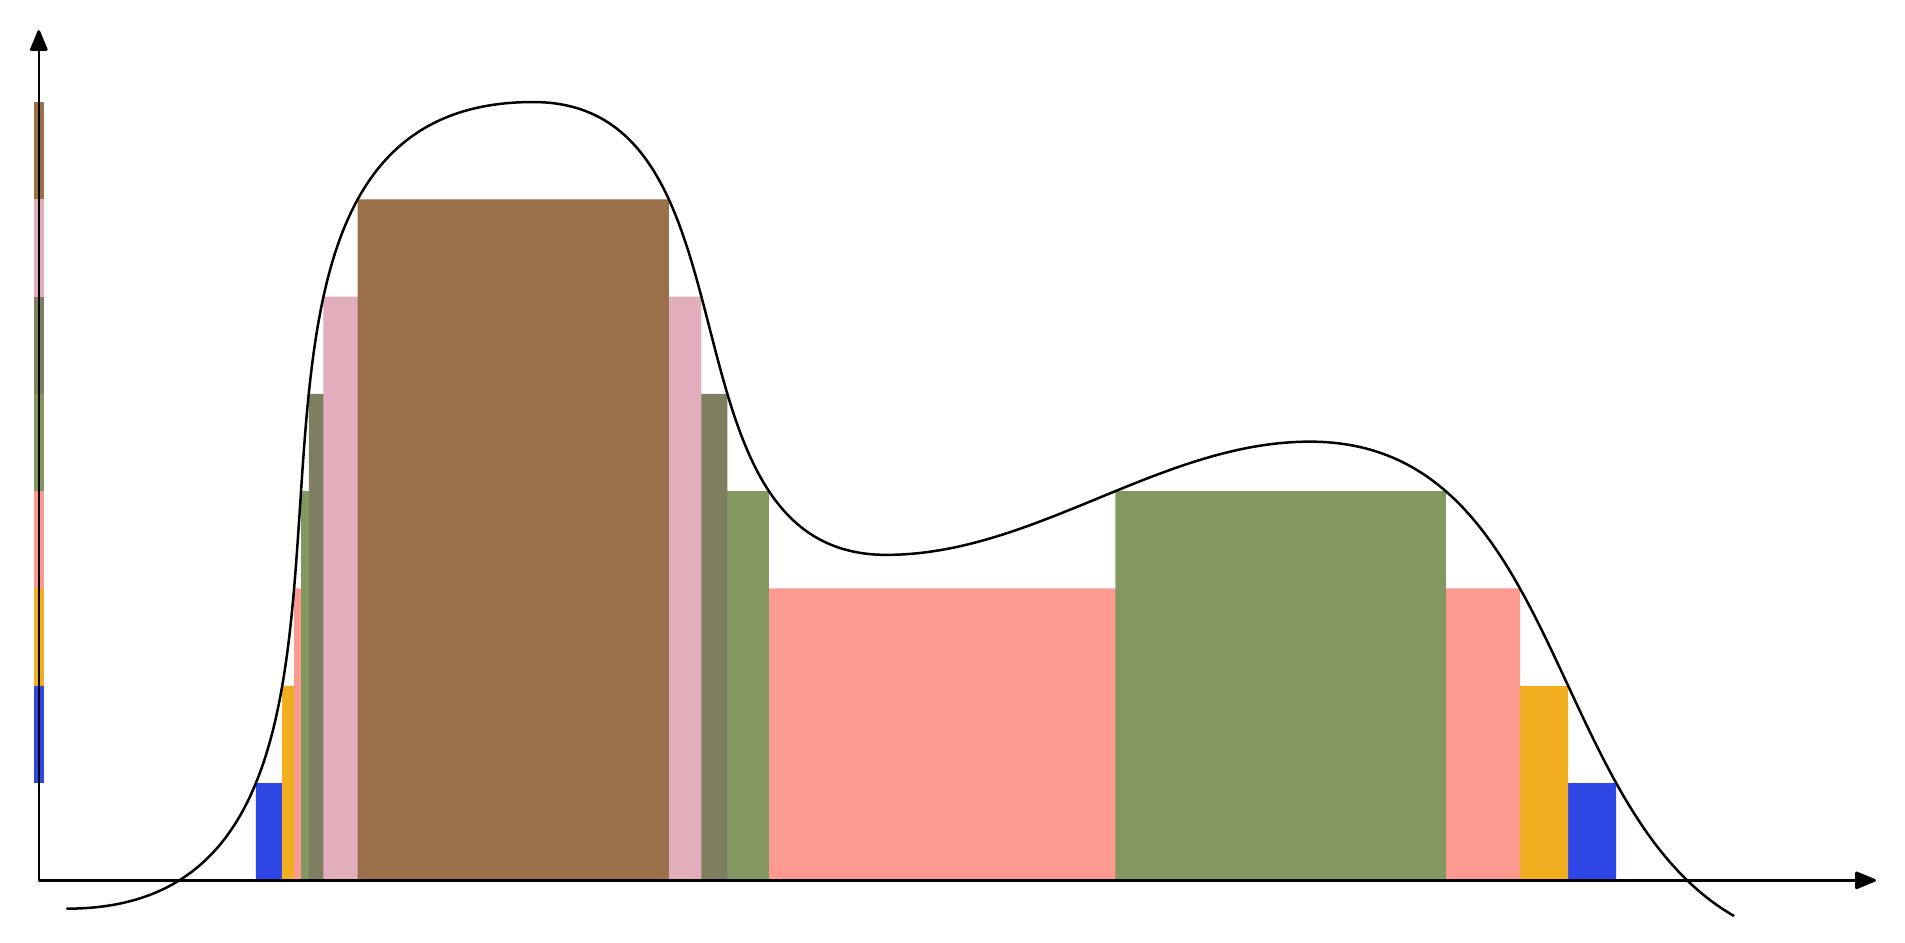
\includegraphics[width=1\linewidth]{fig1}
	\caption{$\varphi_7$.}
	\label{fig:simple-functions1}
\end{subfigure}
\\
	\begin{subfigure}{\linewidth}
	\centering
	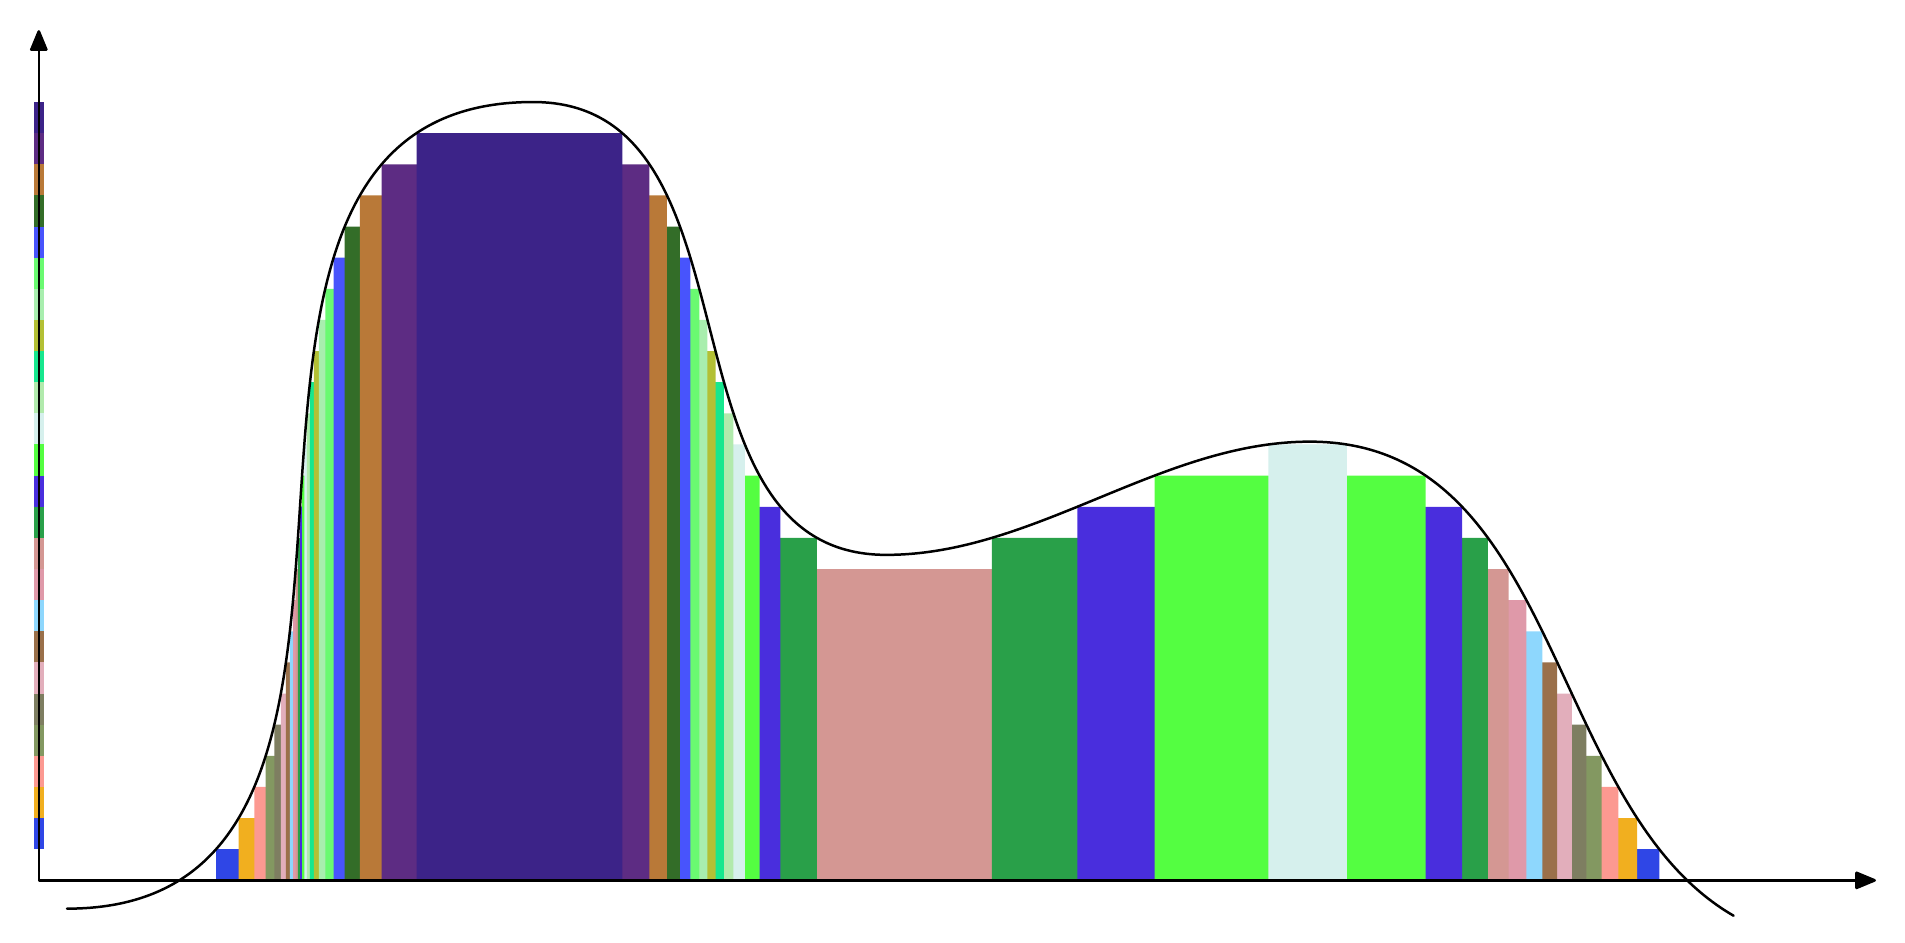
\includegraphics[width=1\linewidth]{fig2}
	\caption{$\varphi_{24}$.}
	\label{fig:simple-functions2}
\end{subfigure}
\end{center}
\caption{\href{https://tex.stackexchange.com/questions/667646/lebesgue-integral-on-tikz}{Approximation by simple functions.}}
\end{figure}
		
		\begin{prop}
			Let $(X,\mathcal{M},\mu)$ be a measure space and let $(X,\overline{\mathcal{M}},\overline{\mu})$ be its completion. If $f$ is a $\overline{\mathcal{M}}$-measurable function on $X$, there is an $\mathcal{M}$-measurable function $g$ such that $f=g\overline{\mu}$-almost everywhere.
		\end{prop}
		
		%RIEMANN VS LEBESGUE INTEGRAL FIGRURE
		\iffalse
		\begin{figure}[H]
			\begin{subfigure}{0.5\linewidth}
				\begin{center}
				\[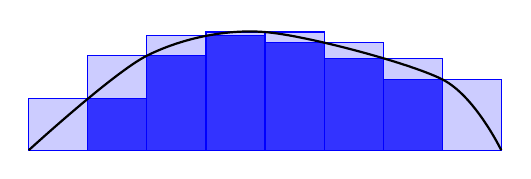
\begin{tikzpicture}
					\begin{scope}[scale=1.5]
						\draw[thick,name path=A] plot[smooth] coordinates {(0,0) (1,0.8) (2,1) (3.5,0.6) (4,0)};
						\begin{scope}[on background layer]
							\foreach \X [count=\Z] in {0,0.5,...,4}
							{\path[name path global=v-\Z,overlay] (\X,0) --  (\X,0|-current bounding box.north);
								\draw[name intersections={of=A and v-\Z,by=i-\Z},blue,fill=blue!20] 
								\ifnum\Z>1
								let \p1=(i-\the\numexpr\Z-1),\p2=(i-\Z) in
								(\X-0.5,0) rectangle (\X,{max(\y1,\y2)})
								\fi;
								\draw[name intersections={of=A and v-\Z,by=i-\Z},blue,fill=blue!80] 
								\ifnum\Z>1
								let \p1=(i-\the\numexpr\Z-1),\p2=(i-\Z) in
								(\X-0.5,0) rectangle (\X,{min(\y1,\y2)})
								\fi;}
						\end{scope}
					\end{scope}
				\end{tikzpicture}\]
				\caption{Riemann integral}
			\end{center}
			\end{subfigure}
			\begin{subfigure}{0.5\linewidth}
				\begin{center}
					\[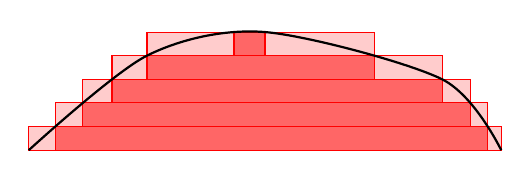
\begin{tikzpicture}
						\begin{scope}[yshift=-2cm,scale=1.5]
							\draw[thick,name path=B] plot[smooth] coordinates {(0,0) (1,0.8) (2,1) (3.5,0.6) (4,0)};
							\begin{scope}[on background layer]
								\foreach \Y [count=\Z] in {0,0.2,0.4,0.6,0.8,1}
								{\path[name path global=h-\Z,overlay] (0,\Y) --  (4,\Y);
									\draw[name intersections={of=B and h-\Z,by={i-\Z-1,i-\Z-2}},red,fill=red!20] 
									\ifnum\Z>1
									let \p1=(i-\the\numexpr\Z-1\relax-1),\p2=(i-\the\numexpr\Z-1\relax-2),
									\p3=(i-\Z-1),\p4=(i-\Z-2)
									in
									({min(\x1,\x3)},\Y-0.2) rectangle ({max(\x2,\x4)},\Y)
									\fi;
									\draw[name intersections={of=B and h-\Z,by={i-\Z-1,i-\Z-2}},red,fill=red!60] 
									\ifnum\Z>1
									let \p1=(i-\the\numexpr\Z-1\relax-1),\p2=(i-\the\numexpr\Z-1\relax-2),
									\p3=(i-\Z-1),\p4=(i-\Z-2)
									in
									({max(\x1,\x3)},\Y-0.2) rectangle ({min(\x2,\x4)},\Y)
									\fi;
								}
							\end{scope}
						\end{scope}
					\end{tikzpicture}\]
					\caption{Lebesgue integral}
				\end{center}
			\end{subfigure}
		\end{figure}
		\fi
		\end{proof}
		
		\subsection{Riesz and Nagy's Functional Analysis}
		This section is a short digression to show the approach of \cite{riesz}.
		\begin{thm}[Lebesgue]
			Every monotonic function $f(x)$ posses a finite derivative at every point with the possible exception of the points $x$ of a set of measure zero, or, as it is often phrased, almost everywhere.
		\end{thm}
		A set of \textbf{\textit{measure zero}} is a set of values $x$ which can be covered by a finite number or by a denumerable sequence of intervals whose total length is arbitrarly small.
		
		Functions $f(x)$ continuous or not, for which the sum
		\[\sum_{ab}=\sum_1^n|f(x_k)-f(x_{k-1})|\]
		defined in terms of a decomposition of the interval $(a,b)$ into partial intervales $(x_{k-1},x_k)\;k=1,2,\ldots,n$, does not surpass a finit bound, independant of the particular choice of decomposition, are called \textbf{\textit{functions of bounded variation}}. The least upper bound is called the \textbf{\textit{total variation of $f(x)$ in the interval $(a,b)$}}.
		\begin{thm}[Lebesgue]
			Every function of bounded variation posses a finite derivative almost everywhere.
		\end{thm}
		\begin{thm}[Fubini]
			Let
			\[f_1(x)+f_2(x)+\ldots=s(x)\]
			be a convergent series all of whose terms are monotonic functions of the same type, defined on the interval $a\leq x\leq b$. Then
			\[f'_1(x)+f'_2(x)+\ldots=s'(x)\]
			except perhaps on a set of measure zero; that is, term by term differentiation is possible almost everywhere.
		\end{thm}
		\begin{thm}[Lebesgue]
			Almost all points of an arbitrary linear set are density points of that set.
		\end{thm}
		We include the following quote regarding Riemann integrals:
		\begin{quotation}[p. 23]
			\textit{(...) we arrive at a necessary condition that $f(x)$ be integrable in the Riemann sense, namely, that the function $f(x)$ be continuous almost everywhere.}
		\end{quotation}
		A \textbf{\textit{step function}} defined on an interval $(a,b)$ is a function having a constant value $c_k$ in each of a finite number of intervals $i_k$ of finite lenght $|i_k|$ and vanishing outside these intervals. We suppose the integral defined for these functions, as usual, by the sum $\sum c_k|i_k|$.
		\begin{lemma}\label{lemma:stepfunctionsA}
			For every sequence $\{\varphi_n(x)\}$ of step functions which decreases to 0 almost everywhere, the sequene of values of their integrals also tends to zero.
		\end{lemma}
		\begin{lemma}\label{lemma:stepfunctionsB}
			If for an increasing sequence of step functions $\{\varphi_n(x)\}$ the values of their integrals have a common bound, then the sequence $\{\varphi_n(x)\}$ tends almost everywhere to a finite limit.
		\end{lemma}
		Denote the class of stepfunctions by $C_0$ and the class of functions which are limits almost everywhere of the sequences $\{\varphi_n\}$ referred to in \cref{lemma:stepfunctionsB}. For $f(x)=\lim\varphi_n(x)$ define
		\[\int_a^bf(x)dx=\lim_{n\to \infty}\int_a^b\varphi_n(x)dx\]
		which does not depend on the particular choice of functions $\varphi_n$. In fact, if $\{\psi_n\}$ is increases almost everywhere to a limit function $g(x)\geq f(x)$, we also have
		\[\lim_{n\to\infty}\int_a^b\psi_n(x)dx\geq\lim_{n\to\infty}\int_a^b\varphi_n(x)dx\]
		so that if $g(x)=f(x)$ almost everywhere is implied.
		\subsection{Integration}
		In this section (\textbf{in progress}) we continue reading \cite{folland}.
		
		The \textbf{\textit{integral of a simple function}} is . The \textbf{\textit{integral of a measurable function}} .
		\begin{thm}[Monotone convergence]
			content...
		\end{thm}
		\begin{thm}[Dominated convergence]
			content...
		\end{thm}
		\begin{prop}[Aditivity of the integral]
			content...
		\end{prop}
		\item The \textbf{\textit{Lebesgue integral}} is the integral we have developed then the measure is the Lebesgue measure.
		\begin{thm}[Fubini-Tonelli]\leavevmode
			\begin{enumerate}
				\item \[\int fd(\mu\times\nu)=\int\left(\int f(x,y)d\nu(y)\right)d\mu(x)=\int\left(\int f(x,y)d\mu(x)\right)d\nu(y)\]
				\item 
			\end{enumerate}
		\end{thm}
		\begin{thm}[2.44]
			\[\int \int f(x)dx=|\det T|\int f\circ T(x)dx\]
		\end{thm}
		\begin{thm}[2.47, diffeomorphisms]
			content...
		\end{thm}

		\end{itemize}
%		\end{itemize}

\clearpage

\section{Point set topology}
	 \subsection{Metric spaces} A \textbf{\textit{metric}} on a set $X$ is a function $\rho:X\times X\to [0,\infty)$ such that
	\begin{enumerate}
		\item $\rho(x,x)=0$ if and only if $x=0$.
		\item $\rho(x,y)=\rho(y,x)$ for all $x,y\in X$.
		\item $d(x,z)\leq d(x,y)+d(y,z)$ for all $x,y,z\in X$.
	\end{enumerate}
	Two metrics $\rho_1$ and $\rho_2$ on a set $X$ are \textbf{\textit{equivalent}} if $C\rho_1\leq\rho_2\leq C'\rho_2$ for some $C,C'>0$.
	
	\begin{thm}Let $(X,d)$ and $(Y,d')$ be metric spaces. If $f:X\to Y$, the following are equivalent conditions for $f$ to be \textbf{\textit{continuous}}:
		\begin{enumerate}
			\item $\forall x\in X\forall\varepsilon>0\exists\delta>0:f(B_\delta(x))\subseteq B_\varepsilon(f(x))$
			\item $\forall x\in X\forall x_n\to x:f(x_n)\to f(x)$.
			\item $\forall F\subseteq Y$ open, $f^{-1}(F)$ is open.
			\item $\forall F\subseteq Y$ closed, $f^{-1}(F)$ is closed.
		\end{enumerate}
	\end{thm}
	If $f:(X,\rho)\to(Y,\rho')$ is such that
	\[\forall\varepsilon>0\exists\delta>0\forall x\in X:f(B_\delta(x))\subseteq B_\varepsilon(f(x))\]
	we say $f$ is \textbf{\textit{uniformly continuous}}.
	\begin{exer*}
		If $(Y,\rho')$ is complete and $f:A\to Y$ is uniformly continuous on $A\subset X$ and $\overline{A}=X$, then $f$ has a unique continuous extension $g:X\to Y$ which is uniformly continuous on $X$. Show that this is not true in general if $Y$ is not complete.
	\end{exer*}
	If $f:(X,\rho)\to(Y,\rho')$ is a bijective function such that for any $x,y\in X$, $\rho(x,y)=\rho'(f(x),f(y))$ we say $f$ is an \textbf{\textit{isometry}} and the two spaces are \textbf{\textit{isometric}}. A function $f:(X,\rho)\to (X,\rho)$ is a \textbf{\textit{contraction}} if there exists a $0<a<1$ such that $\rho(f(x),f(y))\leq a\rho(x,y)$ for any $x,y\in X$. Every contraction is continuous, and if $X$ is complete then any contraction has a unique fixed point.
	
	A sequence $\{x_n\}$ in $X$ \textbf{\textit{converges}} to $x$ if $\lim_{n\to\infty}\rho(x_n,x)=0$. A sequence $\{x_n\}$ in $X$ is called \textbf{\textit{Cauchy}} if $\lim_{n,m\to\infty}\rho(x_n,x_m)=0$, that is
	
	\[\forall\varepsilon>0\exists N\in\N\forall n,m>N:\rho(x_n,x_m)<\varepsilon.\]
	
	A subset $E\subseteq X$ is \textbf{\textit{complete}} if every Cauchy sequence in $E$ converges to its limit in $E$. If $(X,\rho)$ and $(X^*,\rho^*)$ are metric spaces and
	\begin{enumerate}
		\item $(X,\rho)$ is isometric to a subspace $(X,\rho^*)$ of $(X^*,\rho^*)$,
		\item The closure of $X_0$ is all of $X^*$ ($X_0$ is \textbf{\textit{everywhere dense}} or simply \textbf{\textit{dense}}),
	\end{enumerate}
	we say $(X^*,\rho^*)$ is the \textbf{\textit{completion}} of $(X,\rho)$.
	\begin{thm}
		Every metric space $(X,\rho)$ has a completion $(X^*,\rho^*)$. If $(X^{**},\rho^{**})$ is also a completion of $(X,\rho^*)$, then $(X^*,\rho^*)$ is isometric to $(X^{**},\rho^{**})$; that is, the completion of a space is unique up to isometry.
	\end{thm}
	\begin{proof}
		Consider equivalence classes of Cauchy sequences.
	\end{proof}
	
	\begin{prop}
		A closed subset of a metric space is complete, and a complete subset of an arbitrary metric space is closed.
	\end{prop}
	
	\begin{thm}
		If $E$ is a subset of a metric space $(X,\rho)$, the following are equivalent:
		\begin{enumerate}
			\item $E$ is complete and \textbf{\textit{totally bounded}} (it can be covered by finitely many balls of radius $\varepsilon$).
			\item \textbf{(Bolzano-Wierstrass Property.)} Every sequence in $E$ has a subsequence that converges to a point in $E$.
			\item \textbf{(Heine-Borel Property)} If $\{V_\alpha\}_{\alpha\in A}$ is an open cover of $E$, then there is a finite subset $F\subseteq A$ such that $\{V_\alpha\}_{\alpha\in F}$ covers $E$.
		\end{enumerate}
		A set that satsifies any of these condition
		s is called \textbf{\textit{compact}}.
	\end{thm}
	\begin{thm}
		If $(X,\rho)$ is a metric space and $A$ is compact, then $A$ is closed and bounded.
	\end{thm}
	If $(X,\rho)$ is a metric space, $A\subseteq X$ is \textbf{\textit{relatively compact}} if $\overline{A}$ is compact. If $\varepsilon>0$, a subset $N\subset X$ is an \textbf{\textit{$\varepsilon$-net with respect to $A$}} if $\forall x\in A\exists n\in N:\rho(x,n)<\varepsilon$. $A$ is \textbf{\textit{totally boundad}} if for any $\varepsilon>0$ there exists a finite $\varepsilon$-net with respect to $A$.
	
	\begin{thm}
		Let $(X,\rho)$ be a metric space and $A\subseteq X$. If for every sequence of points from $A$ one can select a convergente subsequence, then $A$ is totally bounded.
	\end{thm}
	A set $A$ is \textbf{\textit{countably compact}} if every infinite subset of $A$ has a limit point in $A$. All compact sets are countably compact. $A$ is \textbf{\textit{sequentially compact}} if every sequence in $A$ has a subsequence that converges to a point in $A$. In a metric space, compactness is equivalent to countable and sequential compactness.
	
	\begin{thm} Let $(X,\rho)$ be a metric space and $A\subseteq X$.
		\begin{enumerate}
			\item $A$ is relatively compact if and only if a convergent subsequence can be selected from every sequence of points in $A$. (We do not claim that the limit point is a member of $A$.)
			\item If $A$ is relatively compact, it is also totally bounded.
			\item If $(X,\rho)$ is complete and $A$ is totally bounded, then $A$ is relatively compact.
			\item If $A$ is compact then $A$ is closed and totally bounded.
		\end{enumerate}
	\end{thm}
	
	\subsection{Topological spaces}
	Let $X$ be a nonempty set. A \textbf{\textit{topology}} on $X$ is a family $\mathcal{T}$ of subsets of $X$ that contains $\varnothing$ and $X$ and is closed under arbitrary unions and finite intersections. (That is, if $\{U_\alpha\}_{\alpha\in X}\subset\mathcal{T}$ then $\bigcup_{\alpha\in A}U_\alpha\in\mathcal{T}$ and if $U_1,\ldots, U_n\in\mathcal{T}$ then $\bigcap_{j=1}^nU_j\in\mathcal{T}$.) The pair $(X,\mathcal{T})$ is called a \textbf{\textit{topological space}}.
	
	The memebers of $\mathcal{T}$ are called \textbf{\textit{open sets}} and their complements are called \textbf{\textit{closed sets}}. If $A\subseteq X$, the union of all open sets contained in $A$ is called the \textbf{\textit{interior}} of $A$, denoted by $A^o$; so that a point $x\in A^o$ when there is an open set $O$ contained in $A$ such that $x\in O$. The intersection of all closed sets containing $A$ is called the \textbf{\textit{closure}} of $A$. The difference $\bar{A}\backslash A^o=\bar{A}\cap\overline{A^c}$ is called the \textbf{\textit{boundary}} of $A$ and is denoted by $\partial A$.
	
	Following \cite{narici}, a point $x\in X$ is an \textbf{\textit{adherence point}} of the subset $E$ if every open set containing $x$ conatins a point of $E$. The set of all adherence points of $E$ is called the \textbf{\textit{closure}} of $E$ and it is denoted by $\overline{E}$. It is immediate that $E\subset\overline{E}$.
	\begin{prop}
		Let $X$ be a topological space and $A$ and $B$ subsets of $X$. Then
		\begin{enumerate}
			\item $A\subset B\implies\bar{A}\subset\bar{B}$.
			\item $\overline{A\cup B}\implies\bar{A}\cup\bar{B}$,
			\item $\bar{A}=\bar{\bar{A}}$.
			\item A subset $F$ of $X$ is closed if and only if $F=\overline{F}$.
		\end{enumerate}
	\end{prop}
	If $X$ is a topological space and $A$ is a subset of $X$, a point $x\in X$ is called a \textbf{\textit{limit point}} of $A$ if every open set containing $x$ contains a point of $A$ distinct from $x$. The set of all limit points of $A$ is denoted by $A'$ and is called the \textbf{\textit{derived set of $A$}}. Clearly, $\bar{A}=A\cup A'$, and, in view of the last item in the last proposition, $A$ is closed if and only if $A'\subset A$.
	
	A sequence of points $\{x_n\}$ in a topological space $X$ \textbf{\textit{converges}} to the point $x\in X$ if for every open set $O$ containing $x$ there exists an index $N$ (dependending on $O$) such that $x_n\in O$ for all $n>N$. That is, every open set containing $x$ must contain almost all (but a finite number) of the $x_n$.
	
	\begin{prop} Let $X_1$, $X_2$ and $X_3$ be topologial spaces. Let $f:X_1\to X_2$ and $g:X_2\to X_3$ be mappings.
		\begin{enumerate} 
			\item If $f$ and $g$ are continuous, then the composite mapping $gf$ is continuous.
			\item $f$ is continuous if and only if for every subset $A$ of $X$, $f\bar{A}\subset\overline{f(A)}$.
			\item Suppose $f$ is a 1:1, onto mapping. Then $f$ is a homeomorphism of $X_1$ onto $X_2$ is and only if, for all subsets $A$ of $X_1$, $f(\bar{A})=\overline{f(A)}$.
		\end{enumerate}
	\end{prop}
	
	
	If $\mathcal{T}_1$ and $\mathcal{T}_2$ are two topologies on a set $X$, we say $\mathcal{T}_1$ is \textbf{\textit{weaker}} (or \textbf{\textit{coarser}}) and $\mathcal{T}_2$ \textbf{\textit{stronger}} (or \textbf{\textit{finer}}). $E\subseteq X$ is called \textbf{\textit{dense}} if $\overline{E}=X$ and \textbf{\textit{nowhere dense}} if $\overline{E}$ has empty interior. $X$ is called \textbf{\textit{separable}} if it has a countable dense subset. 
	
	\begin{enumerate}
		\item[$\operatorname{T}_0$] If $x\neq y$, there is an open set containing $x$ but not $y$, or an open set containing $y$ but not $x$.
		\item[$\operatorname{T}_1$] If $x\neq y$, there is an open set containint $y$ but not $x$. Equivalently, $\{x\}$ is closed for every $x\in X$.
		\item[$\operatorname{T}_2$] \textbf{(Hausdorff.)} If $x\neq y$ there are disjoint open sets $U$ and $V$ such that $x\in U$ and $y\in V$.
		\item[$\operatorname{T}_3$] \textbf{(Regular.)} $X$ is $\operatorname{T}_1$ and for any closed set $A\subset X$ and any $x\in A^c$ there are disjoint open sets $U,V$ with $x\in U$ and $a\subseteq V$.
		\item[$\operatorname{T}_{3\frac{1}{2}}$] \textbf{(Tychonoff, Completely regular.)} $X$ is $\operatorname{T}_1$ and for each closed $A\subseteq X$ and each $x\notin A$ there exists $f\in C(X,[0,1])$ such that $f(x)=1$ and $f=0$ on $A$.
		\item[$\operatorname{T}_4$] \textbf{(Normal.)} $X$ is $T_1$ and for any disjoint closed sets $A,B$ in $X$ there are disjoint open sets $U,V$ with $A\subseteq U$ and $B\subseteq V$.
	\end{enumerate}
	
	If $X$ is any set and $\{f_\alpha:X\to Y_\alpha\}_{\alpha\in A}$ is a family of maps from $X$ into some topological spaces $Y_\alpha$, there is a unique weakest topology $\tau$ on $X$ that makes all the $f_\alpha$ continuous called the \textbf{\textit{weak topology generated by $\{f_\alpha\}_{\alpha\in A}$}}. An example of this topology is the \textbf{\textit{product topology}} on $X=\prod_{\alpha\in A}X_\alpha$ with the projections.
	
	\begin{prop}\leavevmode
		\begin{itemize}
			\item If $X_\alpha$ is Hausdorff for each $\alpha\in A$ then $X=\prod_{\alpha\in A}$ is Hausdorff.
			\item If $X_\alpha$ and $Y$ are topological spaces, a function $f:Y\to X=\prod_{\alpha\in A}X_\alpha$ is continuous if and only iff $\pi_\alpha\circ f$ is continuous for each $\alpha$.
			\item If $X$ is a topological space, $A$ is a nonempty set and $\{f_n\}$ is a sequence in $X^A$, then $f_n\to f$ in the product topology if and only if $f_n\to f$ pointwise.
		\end{itemize}
	\end{prop}
	
	If $X$ is any set and $K=\R$ or $\C$, denote by $B(X,K)$ the \textbf{\textit{set of bounded $K$-valued functions on $X$}}, $C(X,K)$ the set of \textbf{\textit{continuous $K$-valued functions on $X$}}, and $BC(X,K)$ the \textbf{\textit{set of bounded continuous functions on $X$}}. If no field is specified we take it to be $\C$.
	
	For $f\in B(X)$ define the \textbf{\textit{uniform norm}} of $f$ to be
	\[\Vert f\Vert_u=\sup\{|f(x)|:x\in X\}\]
	Then the function $\rho(f,g)=|Vert f-g|Vert_u$ is a metric on $B(X)$. Convergence in this metric is simply uniform convergence:
	\[\{f_n\}\overset{u}{to}f\iff\forall\varepsilon>0\exists N\in\N\forall n>N\forall x\in X:|f_n(x)-f(x)|<\varepsilon\]
	$B(X)$ is complete with this metric since $\C$ is complete.
	
	\begin{prop}
		If $X$ is a topological space, $BC(X)$ is a closed subspace of $B(X)$ in the uniform metric; in particular $BC(X)$ is complete.
	\end{prop}
	\begin{lemma}[Urysohn]
		Let $X$ be a normal space. If $A$ and $B$ are disjoint closed sets in $X$, there exists $f\in C(X,[0,1])$ such that $f=0$ on $A$ and $f=1$ on $B$.
	\end{lemma}
	\begin{thm}[Tietze Extension Theorem]
		Let $X$ be a normal space. If $A$ is a closed subset of $X$ and $f\in C(A,[a,b])$, there exists $F\in C(X,[a,b])$ such that $F|A=f$.
	\end{thm}
	\begin{coro}
		If $X$ is normal, $A\subseteq X$ is closed and $f\in C(A)$, there exists $F\in C(X)$ such that $F|A=f$.
	\end{coro}
	Urysohn's lemma shows that every $\operatorname{T}_4$ space is completely regular ($\operatorname{T}_{3\frac{1}{2}}$).
	\begin{thm}[Dugundji]
		Sea $X$ un espacio metrizable, $A=\bar{A}\subset X$ y $L$ un espacio vectorial localmente convexo, y $V\subset L$ convexo. Entonces cualquier función $f:A\to V$ admite una extensión $F$.
		\[\begin{tikzcd}
			A\arrow[r,"f"]\arrow[hook,d]&V\\
			X\arrow[ur,dashed,"F",swap]
		\end{tikzcd}\]
		Además $\img F\subset\operatorname{conv}\img F$.
	\end{thm}
	
		\subsection{Compact spaces}
	
		A topological space $X$ is called \textbf{\textit{compact}} if whenever $\{U_\alpha\}_{\alpha\in A}$ is an open cover of $X$ there is a finite subset $B$ of $A$ such that $X=\bigcup_{\alpha\in B}U_\alpha$. A subset $Y\subseteq X$ is called \textbf{\textit{compact}} if it is compact in the relative topology and \textbf{\textit{precompact}} if its closure is compact.
		
		A family $\{F_\alpha\}_{\alpha\in A}$ of subsets of $X$ has the \textbf{\textit{finite intersection property}} if $\bigcap_{\alpha\in B}F_\alpha\neq\varnothing$ for all finite $B\subseteq A$.
		
		\begin{prop}\leavevmode
			\begin{itemize}
				\item A topological space $X$ is compact if and only if for every family $\{F_\alpha\}_{\alpha\in A}$ of closed sets with the finite intersection property, $\bigcap_{\alpha\in A}F_\alpha\neq\varnothing$.
				\item A closed subset of a compact space is compact.
				\item If $K$ is a compact subset of a Hausdorff space $X$ and $x\notin K$ then there are disjoint open sets $U,V$ such that $x\in U$ and $K\subseteq V$.
				\item Every compact subset of a Hausdorff space is closed.
				\item Every compact Hausdorff space is normal.
				\item If $X$ is compact and $f:X\to Y$ is continuous then $f(X)$ is compact.
				\item If $X$ is compact, then $C(X)=BC(X)$.
				\item If $X$ is compact and $Y$ is Hausdorff, then any continuous bijection $f:X\to Y$ is an homeomorphism.
			\end{itemize}
		\end{prop}
		A topological space $X$ is \textbf{\textit{countably compact}} if every countable open cover of $X$ has a finite subcover, and \textbf{\textit{sequentially compact}} if every sequence in $X$ has a convergent subsequence. For metric spaces compactness and sequential compactness are the equivalent. There exists no general relation between compactness and sequential compactness.
		
		\subsection{Locally Compact Hausdorff spaces}
		
		A topological space is called \textbf{\textit{locally compact}} if every point has a compact neighbourhood (a set $A\subset X$ such that $x\in A^o$). We call locally compact Hausdorff spaces \textbf{\textit{LCH}} for short.
		\begin{prop}Let $X$ be a LCH space.
			\begin{itemize}
				\item If $U\subseteq X$ is open and $x\in U$, there is a compact neighbourhood $K$ of $x$ such that $K\subset U$.
				\item If $K\subseteq U\subseteq X$, with $K$ compact and $U$ open, there exists a precompact open $V$ such that $K\subseteq V\subset \overline{V}\subset U$.
				\item \textbf{(Urysohn's Lemma, Locally Compact Version.)} If $K\subset U\subseteq X$, there exists $f\in C(X,[0,1])$ such that $f=1$ on $K$ and $f=0$ outside a compact subset of $U$.
				\item Every LCH space is completely regular.
				\item \textbf{(Tietze Extension Theorem, Locally Compact Version)} If $K\subseteq X$ is compact and $f\in C(K)$, there exists $F\in C(X)$ such that $F|K=f$. $F$ may be taken to vanish outside a compact set.	
			\end{itemize}
		\end{prop}
		 If $f\in C(X)$, the \textbf{\textit{support of $f$}} is the closure of $\{x\in X:f(x)\neq0\}$ and denote $C_c(X):=\{f\in C(X):\operatorname{supp}f\text{ is compact}\}$. We say $f$ \textbf{\textit{vanishes at infinity}} if for every $\varepsilon>0$ the set $\{x:|f(x)|\geq\varepsilon\}$ is compact and define $C_0(X):=\{f\in C(X):f\text{ vanishes at infinity}\}$.
		 \begin{prop}
		 	If $X$ is an LCH space, $C_0(X)$ is the closure of $C_c(X)$ in the uniform metric.
		 \end{prop}
		 If $X$ is a topological space, there are many ways of topologizing $\C^X$. One way is the product topology, that is, the topology of pointwise convergence. Another is the \textbf{\textit{topology of uniform convergence}}, which is generated by the sets
		 \[\left\{g\in\C^X:\sup_{x\in X}|g(x)-f(x)|<n^{-1}\right\}\qquad n\in\N,f\in\C^X.\]
		 In view of a previous proposition (cite?), we know $C(X)$ is a closed subset of $\C^X$ with the topology of uniform convergence. Another topology is the \textbf{\textit{topology of uniform convergence on compact sets}}, generated by the sets
			 \[\left\{g\in\C^X:\sup_{x\in K}|g(x)-f(x)|<n^{-1}\right\}\qquad n\in\N,f\in\C^X,K\subseteq X\text{ compact}.\]
		\begin{prop}Let $X$ be an LCH space.
			\begin{itemize}
				\item If $E\subseteq X$, then $E$ is closed if and only if $E\cap K$ is closed for every compact $K\subseteq X$.
				\item $C(X)$ is a closed subspace of $\C^X$ in the topology of uniform convergence on compact sets.
				\item If $\{U_j\}_{j=1}^n$ is an open cover of a compact subset $K$ of $X$, then there is a partition of unity on $K$ subordinate to $\{U_j\}_{j=1}^n$ soncisting of compactly supported functions.
			\end{itemize}
		\end{prop}
		
		\begin{thm}[Urysohn Metrization Theorem]
			Every second countable normal space is metrizable.
		\end{thm}
		
		\subsection{Three compactness theorems}
		
		Recall that if $X=\prod_{\alpha\in A}X_\alpha$, an element $x\in X$ is just a mapping from $A$ to $\bigcup_{\alpha\in A}X_\alpha$, with $x(\alpha)$ the $\alpha$th coordinate of $x$.
		
		\begin{thm}
			If $\{X_\alpha\}_{\alpha\in A}$ is a family of compact topological spaces, then $X=\prod_{\alpha\in A}X_\alpha$ is compact with the produc topology.
		\end{thm}
		Let $X$ be a topological space and $\mathcal{F}\subseteq C(X)$ a family of complex-valued continuous functions on $X$. We say $\mathcal{F}$ is \textbf{\textit{equicontinuous at $x\in X$}} if for every $\varepsilon>0$ there is a neighbourhood $U$ of $x$ such that $|f(x)-f(y)|<\varepsilon$ for all $y\in U$ and all $f\in\mathcal{F}$; and \textbf{\textit{equicontinuous}} if it is equicontinuous at every $x\in X$. Also, $\mathcal{F}$ is \textbf{\textit{pointwise bounded}} if $\{|f(x)|:f\in\mathcal{F}\}$ is bounded for all $x\in X$.
	
		\begin{thm}[Arzelá-Ascoli I]
			Let $X$ be a compact Housdorff space. If $\mathcal{F}$ is an equicontinuous, pointwise bounded subset of $C(X)$, then $\mathcal{F}$ is totally bounded in the uniform metric, and the closure of $\mathcal{F}$ in $C(X)$ is compact.
		\end{thm}
		\begin{thm}[Arzelá-Ascoli II]
			Let $X$ be a locally compact Housdorff space. If $\{f_n\}$ is an equicontinuous, pointwise bounded sequence in $C(X)$, then there exists $f\in C(X)$ and a subsequence of $\{f_n\}$ that converges to $f$ uniformly on compact sets.
		\end{thm}

		\subsection{The Stone-Weierstrass Theorem}
		Recall that the Weierstrass theorem states that any continuous function on a compact interval $[a,b]$ is the uniform limit of polynomials on $[a,b]$. Throughout this subsection, $X$ will denote a compact Hausdorff space, and $C(X)$ is equipped with the uniform metric.
		
		A subset $\mathcal{A}$ of $C(X,\R)$ of $C(X)$ is said to \textbf{\textit{separate points}} if for every $x,y\in X$ with $x\neq y$ there exists $f\in \mathcal{A}$ such that $f(x)\neq f(y)$. $\mathcal{A}$ is called an \textbf{\textit{algebra}} if it is a real (resp. complex) vector subspace of $C(X,\R)$ (resp. $C(X)$) such that $fg\in \mathcal{A}$ whenever $f,g\in\mathcal{A}$. $\mathcal{A}$ is called a \textbf{\textit{lattice}} if $\max (f,g)$ and $\min (f,g)$ are in $\mathcal{A}$ whenever $f,g\in \mathcal{A}$. If $\mathcal{A}$ is an algebra or a lattice, so is its closure in the uniform metric.
		
		\begin{thm}[Stone-Weierstrass Theorem]
			Let $X$ be a compact Hausdorff space. If $\mathcal{A}$ is a closed subalgebra of $C(X,\R)$ that separates points, then either $A=C(X,\R)$ of $\mathcal{A}=\{f\in C(X,\R):f(x_0)=0\}$ for some $x_0\in X$. The first alternative holds if and only if $\mathcal{A}$ contains the constant functions.
		\end{thm}
		\begin{coro}
			Supoose $\mathcal{B}$ is a subalgebra of $C(X,\R)$ that separates points. If there exists $x_0\in X$ such that $f(x_0)=0$ for all $f\in\mathcal{B}$, then $\mathcal{B}$ is dense in $\{f\in C(X,\R):f(x_0)=0\}$. Otherwise, $\mathcal{B}$ is dense in $C(X,\R)$.
		\end{coro}
		The classical Weierstrass approximation theorem is the special case of this corollary where $X$ is the compact subset of $\R^n$ and $\mathcal{B}$ is the algebra of polynomials on $\R^n$ (restricted to $X$); here $\mathcal{B}$ contains the constant functions, so it is dense in $C(X,\R)$.
		
		The Stone-Weirstrass theorem, as stated, is false for complex-valued functions. We may show that $f(z)=\bar{z}$ cannot be approximately uniformly by polynomials on the unit circle.
		
		\begin{thm}[Complex Stone-Weirstrass Theorem]
			Let $X$ be a compact Hausdorff space. If $\mathcal{A}$ is a closed complex subalgebra of $C(X)$ that separates points and is closed under complex conjugation, then either $A=C(X)$ of $\mathcal{A}=\{f\in C(X):f(x_0)=0\}$ for some $x_0\in X$.
		\end{thm}
		Finally, there is a version of the Stone-Weirstrass theorem for noncompact LCH spaces. We state for real functions; the complex analogue is an immediate consequence.
		\begin{thm}[LCH Stone-Weirstrass Theorem]
			Let $X$ be a noncompact LCH space. If $\mathcal{A}$ is a closed complex subalgebra of $C_0(X,\R)$ that separates points, then either $A=C_0(X,\R)$ of $\mathcal{A}=\{f\in C_0(X,\R):f(x_0)=0\}$ for some $x_0\in X$.
		\end{thm}

\clearpage
\section{Inner product spaces}
Let $X$ be a real or complex vector space.
	\subsection{Inner products} An \textbf{\textit{inner product}} on $X$ is a mapping
	\begin{align*}
		\langle-,-\rangle:X\times X\to F
	\end{align*}
	with the following properties:
	\begin{enumerate}
		\item[($\operatorname{I}_1$)] if $x,y\in X$ then $\langle x,y\rangle=\overline{\langle x,y\rangle}$;
		\item[($\operatorname{I}_2$)] if $\alpha,\beta$ are scalars, $\langle\alpha x+\beta y,z\rangle =\alpha\langle x,z\rangle+\beta\langle y,z\rangle$;
		\item[($\operatorname{I}_3$)] $\langle x,x\rangle\geq0$ for all $x\in X$ and equal to zero if and only if $x$ is the zero vector. (Since, by $\operatorname{I}_1$, $\langle x,x\rangle$ must be real.)
	\end{enumerate}
	\begin{examples}\leavevmode
		\begin{enumerate}
			\item Let $X=C[a,b]$ be complex-valued continuous functions on the closed interval $[a,b]$ with pointwise addition and scalar product. As the inner product of any two vectors $f$ and $g$ in this space take
		\[\langle f,g\rangle=\int_a^bf(x)\overline{g(x)}dx\]
		\item Let $X=l_2$, the set of all sequences of complex numbers $(a_1,a_2,\ldots)$ with the property that $\sum_{i=1}^\infty|a_i|^2<\infty$. As the inner product of any two vectors $x=(a_i)$ and $y=(b_i)$ in this space take
		\[\langle f,g\rangle=\sum_{i=1}^\infty a_i\overline{b}_i\]
		which converges by the Hölder inequality.
		
		\item Let $Y$ be the closed interval $[a,b]$, $S$ the Lebesgue measurable sets and $\mu$ the Lebesgue measure. Then, for the equivalence clasess of square-integrable functions (complex-valued) on $[a,b]$ we can take as the inner product of two clases $f$ and $g$,
				\[\langle f,g\rangle=\int_a^bf(x)\overline{g(x)}dx\]
		where the integral is the Lebesgue integral. This space is denoted by $L_2(a,b)$.
		\end{enumerate}
		\end{examples}
		\begin{thm}[Cauchy-Schwarz inequality]
			Let $X$ be an inner product space and let $x,y\in X$. Then
			\[|\langle x,y\rangle\leq\Vert x\Vert\Vert y\Vert\]
			with equality holding if and only if $x$ and $y$ are linearly independent.
		\end{thm}
		\subsection{Orthogonal projections} Two vectors $x,y\in X$ are \textbf{\textit{orthogonal}} if $\langle x,y\rangle=0$.
		\begin{examples}\leavevmode
	\begin{enumerate}
		\item In $L_2(–\pi,\pi)$, the collection (or any subset thereof)
			\[x_n=\frac{1}{\sqrt{2\pi}}e^{int},\qquad n=0,\pm1,\ldots\]
			is an orthonormal set of vectors.
			\begin{proof}
				For any $n\in\Z$,
				\[\int_{-\pi}^\pi x_n\overline{x}_ndt=\frac{1}{2\pi}\int_{-\pi}^\pi e^{int}\overline{e^{int}}dt=\frac{1}{2\pi}\int_{-\pi}^\pi \Vert e^{int}\Vert^2dt=1,\]
				and if $m$ is another integer,
				\[\int_{-\pi}^\pi x_n\overline{x}_mdt=\frac{1}{2\pi}\int_{-\pi}^\pi e^{int}\overline{e^{imt}}dt=\frac{1}{2\pi}\int_{-\pi}^\pi e^{(n-m)it}dt=\frac{1}{2\pi}\left[\frac{e^{(n-m)it}}{(n-m)i}\right]_{-\pi}^\pi=0.\]
			\end{proof}
			\item If we restric out attention to only real-valued functions that are square-integrable on the interval $[-\pi,\pi]$, then the collection (or any subset thereof)
			\begin{align*}
				\frac{1}{\sqrt{2\pi}},&\frac{1}{\sqrt{\pi}}\cos t,\frac{1}{\sqrt{\pi}}\cos 2t,\ldots\\
				&\frac{1}{\sqrt{\pi}}\sin t,\frac{1}{\sqrt{\pi}}\sin 2t,\ldots
			\end{align*}
			is an orthonormal set.
		\end{enumerate}
		\end{examples}
		\begin{thm}
			If $S$ is an orthonoromal subset of an inner product space, then it is linearly independent (where linear independence is defined as finite sums).
		\end{thm}
		\begin{thm}[Gram-Schmidt process]
			Let $X$ be an inner product space. If $\{y_1,y_2,\ldots\}$ is a linearly independent set of vectors, then there exists an orthonormal set of vectors $\{x_1,x_2,\ldots\}$ such that, for any $n$,
			\[\langle y_1,y_2,\ldots,y_n\rangle=\langle x_1,x_2,\ldots,x_n\rangle\]
			where the brackets indicate the subspace spanned by the vectores enclosed.
		\end{thm}
		If $S$ is any subset of $X$, the \textbf{\textit{orthogonal complement of $S$ in $X$}} is the linear space $S^\perp:=\{x\in X:x\perp s\text{ for all }s\in S\}$.
		\begin{thm}
			If $M$ is a finite-dimensional subspace of $X$, then $X=M\oplus M^\perp$.
		\end{thm}
		\subsection{Riesz representation theorem}
	 \begin{thm}[Riesz]
		If $X$ is a finite-dimensional inner product space and $f$ is a linear functional on $X$, then there exists a unique vector $y\in X$ such that $f(x)=\langle x,y\rangle for all x\in X$.
	\end{thm}
	\begin{proof}
		Given an orthonormal basis $e_i$ of $X$, consider $y=\sum_i\overline{f(e_i)}e_i$.
	\end{proof}
	{\color{blue-violet}In Riemannian geometry this is called \textbf{\textit{raising an index}} of a 1-form. Indeed, $\omega_p\in\Lambda^1(T_pM)$ is just a linear functional on $T_pM$, and $(\omega)^\sharp=g^{ij}\omega_{j}E_i$ at $p$ is just a vector $y$ such that $\omega_p(x)=\langle x,y\rangle$ for all $x\in T_pM$. So the former theorem may also be stated as ``$y=f^\sharp$ exists". Recall this is given by viewing the inner product as a nonsingular matrix.}
	
	\subsection{Adjoint operator}
	 Let $A:X\to X$ be a linear transformation in a finite-dimensional inner product space $X$. For a given $y\in X$, define the linear functional
	\begin{align*}
		f^y:X&\to F\\
		x&\mapsto\langle Ax,y\rangle
	\end{align*}
	which, by the Riesz representation theorem yields a unique $z\in X$ such that
	\[f^y(x)=\langle x,z\rangle\]
	Then the \textbf{\textit{adjoint of $A$}} is the linear map
	\begin{align*}
		A^*:X&\to X\\
		y&\mapsto z
	\end{align*}
	so that $\langle Ax,y\rangle=\langle x,A^*y\rangle$.
	\begin{prop}[Properties of the adjoint]\leavevmode
		\begin{enumerate}
			\item $(\alpha A)^*=\overline{\alpha}A^*$.
			\item $(A+B)^*=A^*+B^*$.
			\item $(AB)^*=B^*A^*$.
			\item $(A^*)^*=A$.
		\end{enumerate}
	\end{prop}
	If $A=A^*$ we say $A$ is \textbf{\textit{self-adjoint}}, and if $AA^*=A^*A$ we say $A$ is \textbf{\textit{normal}}.
	\begin{thm}
		If $A$ is self-adjoint, its eigenvalues are real. Eigenvectors associated to distinct eigenvalues of a self-adjoint operator are orthogonal.
	\end{thm}
	\begin{thm}
		If $M$ is an invariant subspace of $X$ under $A$, then $M^\perp$ is invariant under $A^*$.
	\end{thm}
	\begin{thm}
		If $A$ is a linear transformation on a finite-dimensional inner product space $X$, then $\operatorname{range} (A)^\perp=\operatorname{null}(A^*)$.
	\end{thm}
	
	\subsection{Spectral theorem for normal transformations}
	\begin{thm}
		Let $A$ be a self-adjoint transformation in a finite-dimensional inner product space $X$. Then there exists an orthonormal basis of $X$ consistinf of eigenvectors of $A$.
	\end{thm}
	\begin{lemma}
		Let $A$ be a normal transformation in a finite-dimensional inner product space $X$. Then $\Vert Ax\Vert=\Vert A^*x\Vert$ for all $x\in X$.
	\end{lemma}
	\begin{thm}
		Let $A$ be a normal transformation in a complex finite-dimensional inner product space $X$. Then there exists an orthonormal basis of $X$ consistinf of eigenvectors of $A$.
	\end{thm}
	\begin{thm}
		If $A$ is a normal transformation on a finite-dimensional inner product space. Eigenvectors associated to distinct eigenvalues of a self-adjoint operator are orthogonal.
	\end{thm}
	Recall that the notation $X=M_1\oplus\ldots\oplus M_k$ means that $X$ is the \textbf{\textit{direct sum}} of the $M_i$, which means that $X=M_1+\ldots+M_k$ and $M_i\cap\{M_1+\ldots \hat{M_i}+\ldots+M_k\}=\{0\}$, (every element in $X$ is expressed as a unique sum of elements in $M_i$). If $M_i\perp M_j$ for all $i\neq j$, we say this is an \textbf{\textit{orthogonal direct sum decomoposition of $X$}}, and the \textbf{\textit{orthogonal projection to $M_j$}} is just taking the corresponding component of a given element in its decomposition.
	\begin{thm}[Spectral decomposition theorem for normal transformations]
		To every normal transformation $A$ on a complex finite-dimensional inner product space there correspond scalar $\lambda_1,\ldots,\lambda_k$, the distinct eigenvalues of $A$, and orthogonal projections $E_1,\ldots,E_k$ with $k\leq \dim X$, such that
		\begin{enumerate}
			\item $E_i$ is the orthogonal projection on $\operatorname{Null}(A-\lambda_i)$ for $i=1,\ldots,k$.
			\item $E_i\neq0$ and $E_iE_j=0$ for $i,j=1,\ldots,k$.
			\item $\sum_{j=1}^kE_j=1$.
			\item $\sum_{j=1}^k\lambda_jE_j=A$.
		\end{enumerate}
	\end{thm}
	If $A$ was self-adjoint, we could weaken the hypotheses to a real inner product space.

	\subsection{Unitary and orthogonal transformations}
	Let $X$ be a finite-dimensional inner product space, and $U:X\to X$ a linear transformation with $U^*U=1$. We say $U$ is \textbf{\textit{unitary}} if $X$ is complex and \textbf{\textit{orthogonal}} if $X$ is real. The condition $U^*U=1$ implies that $UU^*=1$.
	
	\begin{thm}
		Let $X$ be a finite-dimensional inner product space, and $U:X\to X$ a linear transformation. The following statements are equivalent:
		\begin{enumerate}
			\item $U^*U=1$.
			\item $\langle Ux,Uy\rangle=\langle x,y\rangle$.
			\item $\Vert Ux\Vert=\Vert x\Vert$ for all $x\in X$.
		\end{enumerate}
	\end{thm}
	\begin{thm}
		If $U$ is a unitary transformation on the finite-dimensional inner product space $X$, then each of the eigenvalues of $U$ must have an absolute value equal to 1.
	\end{thm}
	To summarize:
	\begin{thm}
		Let $A$ be a normal transformation on a complex finite-dimensional inner product space. Then
		\begin{enumerate}
			\item $A$ is self-adjoint is and only if each eigenvalue of $A$ is real.
			\item $A$ is unitary if and only if each eigenvalue of $A$ has absolute value equal to 1.
		\end{enumerate}
	\end{thm}

\subsection{Normed spaces}
	Let $X$ be a real or complex vector space. A \textbf{\textit{norm}} on $X$ is a function $\Vert \cdot\Vert:X\to\R$ such that
\begin{enumerate}
	\item $\Vert x\Vert\geq0$ and $\Vert x\Vert=0$ if and only if $x=0$.
	\item $\Vert\lambda x\Vert=|\lambda|\Vert x\Vert$ for all $x\in X$ and $\lambda\in\R$.
	\item \textbf{(Triangle inequality.)} $\Vert x+y\Vert\leq\Vert x\Vert+\Vert y\Vert$ for all $x,y\in X$.
\end{enumerate}
Every normed space is a metric space with the distance function $\rho(x,y)=\Vert x-y\Vert$. Two norms $\Vert\cdot\Vert_1$ and $\Vert\cdot\Vert_2$ are called \textbf{\textit{equivalent}} if there exist $C_1,C_2>0$ such that
\[C_1\Vert x\Vert_1\leq \Vert x\Vert_2\leq \Vert x\Vert_1\qquad\forall x\in X\]
Equivalent norms define the same topology and the same Cauchy sequences.

A normed space that is complete is called a \textbf{\textit{Banach space}}.
\begin{thm}
	For every normed linear space $X$ there is a complete normed linear space $X^*$ such that $X$ is \textbf{\textit{congruent}} (isomorphic and isometric) to a dense subset of $X^*$ and the norm on $X^*$ extends the norm on $X$.
\end{thm}
If $\{x_n\}$ is a sequence in $X$, the series $\sum_{n=1}^\infty x_n$ \textbf{\textit{converges to $x$}} if $\sum_{n=1}^N\to x$ as $N\to \infty$, and it is \textbf{\textit{absolutely convergent}} is $\sum_{n=1}^\infty\Vert x_n\Vert<\infty$.
\begin{thm}
	A normed vector space $X$ is complete if and only if every absoultely convergent series in $X$ converges.
\end{thm}

\begin{examples}\leavevmode
	\begin{itemize}
		\item If $X$ is a topological space, $B(X)$ and $BC(X)$ are Banach spaces with the uniform norm $\Vert f\Vert_u=\sup_{x\in X}|f(x)|$.
		\item If $(X,\mathcal{M},\mu)$ is a measure space, $L^1(\mu)$ is a Banach space with the norm $\Vert f\Vert_1=\int|f|d\mu$. (Observe that $\Vert\cdot\Vert_1$ is only a seminorm if we do not identify functions that are equal a.e.)
		%\item If $(X\mathcal{M})$ is a normed space and $M(X)$ is the space of complex measures on $(X,\mathcal{M})$, then $M(X)$ is a Banach space.
	\end{itemize}
\end{examples}
If $X$ and $Y$ are normed vector spaces, $X\times Y$ is a normed vector space with the \textbf{\textit{product norm}}, $\Vert(x,y)\Vert=\max(\Vert x\Vert,\Vert y\Vert)$.  If $M$ is a vector subspace of $X$, the quotient space $X/M$ consisting of equivalence classes under $x\sim y$ iff $x-y\in M$ is a normed space with the \textbf{\textit{quotient norm}}, $\Vert x+M\Vert=\inf_{y\in M}\Vert x+y\Vert$.

A linear map $T:X\to Y$ between two normed vector spaces is \textbf{\textit{bounded}} if there exists $C\geq0$ such that
\[\Vert Tx\Vert\leq C\Vert x\Vert\qquad \forall x\in X\]
\begin{prop}
	If $X$ and $Y$ are normed vector spaces and $T:X\to Y$ is a linear map, then $T$ is continuous if and only if it is bounded.
\end{prop}
\begin{proof}
	($\implies $) There exists $\delta>0$ such that $\Vert x\Vert\leq\delta$ implies $\Vert Tx\Vert\leq1$. For any nonzero $x\in X$,
	\[\Vert Tx\Vert=\left\Vert \frac{\Vert x\Vert}{\delta}T\left(\delta\frac{x}{\Vert x\Vert}\right)\right\Vert\leq\frac{1}{\delta} \Vert x\Vert.\]
	($\impliedby$) If $\Vert x-y\Vert<\frac{\varepsilon}{C}$,
	\[\Vert T(x)-T(y)\Vert=\Vert T(x-y)\Vert\leq C\Vert x-y\Vert<\varepsilon.\]
\end{proof}
In fact, if $T$ is bounded it is uniformly continuous and even Lipschitz continuous.

We denote by $L(X,Y)$ the space of bounded linear maps from $X$ to $Y$, which is a normed vector space with the \textbf{\textit{operator norm}}
\begin{align*}
	\Vert T\Vert&=\sup_{\substack{x\in X\\\Vert x\Vert\leq1}}\Vert Tx\Vert\\\\
	&=\sup\{\Vert Tx\Vert:\Vert x\Vert=1\}\\
	&=\sup\left\{\frac{\Vert Tx\Vert}{\Vert x\Vert}:x\neq0\right\}\\
	&=\inf\{C:\Vert Tx\Vert\leq C\Vert x\Vert \text{ for all }x\in X\}
\end{align*}
\begin{prop}
	If $Y$ is complete, so is $L(X,Y)$.
\end{prop}
\begin{proof}
	If $\{T_n\}$ is a Cauchy sequence in $L(X,Y)$, the sequence $\Vert T_nx\Vert$ is Cauchy in $Y$ since $\Vert T_nx-T_mx\Vert\leq\Vert T_n-T_m\Vert\Vert x\Vert$. Define pointwise $Tx=\lim_{n\to\infty}T_nx$.
\end{proof}
$T$ is \textbf{\textit{invertible}} if it bijective and $T^{-1}$ is bounded. It is called an isometry if $\Vert Tx\Vert=\Vert x\Vert$ for all $x\in X$. An isometry is injective but not necessarily surjective.

If $X$ is a vector space over $K=\R,\C$, a \textbf{\textit{linear functional}}. is a linear map from $X$ to $K$.

\begin{prop}[Relationship between real and complex linear functionals]
	Let $X$ be a vector space over $\C$. If $f$ is a complex linear functional on $X$,
	$u:=\operatorname{Re}x$ is a real linear functional and $f(x)=u(x)-iu(ix)$.
	Conversely, if $u$ is a real functional on $X$, then $f(x):=u(x)-iu(ix)$ is a complex linear functional, and if $X$ is normed, $\Vert u\Vert=\Vert f\Vert$.
\end{prop}

\section{Hahn-Banach theorems}

\subsection{Analytic form of the Hahn-Banach theorem}
It is not obvious that there are any nonzero bounded linear functionals on an arbitrary normed vector space. If $E$ is a real vector space, \textbf{\textit{sublinear}} or \textbf{\textit{Minkoswky functional}} on $E$ is a map $p:E\to\R$ such that

\begin{equation}\label{eq:sublinear1}
		p(\lambda x)=\lambda p(x)\qquad\forall x\in X\text{ and }\lambda\geq0
\end{equation}
\begin{equation}\label{eq:sublinear2}
	p(x+y)\leq p(x)+p(y)\qquad\forall x,y\in X
\end{equation}

\begin{thm}[Helly-Hahn-Banach]\label{thm:helly-hahn-banach}
	Let $E$ be a vector space over $\R$ and $p:E\to\R$ a sublinear functional. If $G\subseteq E$ is a linear subspace and $g:G\to\R$ is a linear functional such that
	\[g(x)\leq p(x)\quad\forall x\in E,\]
	then there exists a linear functional $f$ defined on all of $E$ that extends $g$, that is, $g(x)=f(x)\;\forall x\in G$ and such that
	\[f(x)\leq p(x)\quad\forall x\in E.\]
\end{thm}
For a proof first recall that a partial order $P$ is \textbf{\textit{inductive}} if every totally ordered subset $Q$ in $P$ has an upper bound, and that
\begin{lemma}[Zorn]
	Every nonempty order set that is inductive has a maximal element.
\end{lemma}
\begin{proof} (Of \cref{thm:helly-hahn-banach})
	Consider the set
	\[P=\left\{h:D(h)\subseteq E\to\R:\substack{D(h)\text{ is a linear subspace of }E,\\
	h\text{ is linear},G\subseteq D(h),\\
	h\text{ extends }g,\text{ and }h(x)\leq p(x)\;\forall x\in D(h)
	}\right\}\]

Then $P$ is a partial order with
\[h_1\leq h_2\iff D(h_1)\subseteq D(h_2)\text{ and }h_2\text{ extends }h_1\]
$P$ is nonempty since $g\in P$. To show it is inductive, take $Q\subseteq P$ a partially order subset and write $Q=(h_i)_{i\in I}$. Then define
\[D(h)=\bigcup_{i\in I}D(h_i),\qquad h(x)=h_i(x)\quad\text{if }x\in D(h_i) \text{ for some }i\in I\]
which is an upper bound of $Q$, so that there is a maximal element $f$ in $P$ by Zorn's Lemma. To finish it suffices to show that $D(f)=E$.

For a contradiction suppose that $D(f)\neq E$ and choose $x_0\notin D(f)$. We shall construct a function $h\in P$ such that $f<h$. Define $D(h)=D(f)+\R x_0$ and, for every $x\in D(f)$, set
 \[h(x+\lambda x_0)=f(x)+t\alpha\quad \forall \lambda\in\R\]
 where $\alpha$ is a constant that we choose as follows. We must ensure that
\[h(x+\lambda x_0)=f(x)+\lambda\alpha\leq p(x+tx_0)\quad\forall x\in D(f)\quad\text{and}\quad\forall \lambda\in\R\]
For any $x,y\in D(f)$,
\begin{align*}
	f(x)+f(y)=f(x+y)\leq p&(x+y)\leq p(x+x_0)+p(y-x_0)\\
	\implies f(x)-p(y-x_0)&\leq p(x+x_0)-f(y)
\end{align*}
So let $\alpha$ satisfy
\[\sup_{y\in D(f)}\{f(y)-p(y-x_0)\}\leq\alpha\leq\inf_{x\in D(f)}\{p(x+x_0)-f(x)\}\]
If $\lambda =0$, then $h(x)=f(x)\leq p(x)$. If $\lambda\neq0$ we must be careful since sublinear functionals only satisfy \cref{eq:sublinear1} for positve scalars.

If $\lambda >0$, then 
\begin{align*}
	h(x+\lambda x_0)&=\lambda\cdot h(x/\lambda+x_0)\\
	&=\lambda\cdot(f(x/\lambda)+\alpha))\\
	&\leq \lambda\cdot(f(x/\lambda)+p(x/\lambda+x_0)-f(x/\lambda))\\
	&\leq p(x+\lambda x_0)
\end{align*}
and if $\lambda=-\mu<0$,
\begin{align*}
	h(x+tx_0)&=(-\lambda)\cdot h(-x/\lambda-x_0)\\
	&=\mu\cdot(f(x/\mu)-\alpha))\\
	&\leq \mu\cdot(f(x/\mu)-f(x/\mu)+p(x/\mu+x_0))\\
	&\leq p(x-\mu x_0)\\
	&=p(x+\lambda x_0).
\end{align*}
Then $h\in P$, $h$ extends $f$ and $D(f)\subsetneq D(h)$, which is impossible since $f$ is maximal.
\end{proof}

An example of a sublinear functional is a \textbf{\textit{seminorm}}, which is a function that satisfies the first two conditions of being norm, but the third. If $p$ is a seminorm, 
\begin{thm}[Complex Hahn-Banach]
	Let $E$ be a complex vector space, $p$ a seminorm on $E$, $G\subseteq E$ a subspace of $E$ and $f$ a complex linear functional on $G$ such that $|g(x)|\leq p(x)\;\forall x\in G$. Then there exists a complex linear functional $f$ defined on all of $E$ that extends $g$ and $|f(x)|\leq p(x)$.
\end{thm}

The space of al continuous linear functionals on $E$, denoted by $E^*:=L(E,K)$, is called the \textbf{\textit{dual space}} of $E$. Since $K$ is complete, $X^*$ is complete with the operator norm. We denote the \textbf{\textit{dual norm}} (it remains for me to check wether this is the same as the operator norm) by
\[\Vert f\Vert_{E^*}=\sup_{\substack{x\in E\\\Vert x\Vert\leq1}}|f(x)|=\sup_{\substack{x\in E\\\Vert x\Vert\leq1}}f(x)\]
Given $f\in E^*$ and $x\in E$ we shall often write $\langle f,x\rangle$ instead of $f(x)$ and call $\langle-,-\rangle$ the \textbf{\textit{scalar product for the duality $E^*,E$}}.
\begin{coro}\label{coro:HB1}
	Let $G\subseteq E$ be a linear subspace. If $g:G\to\R$ is a continuos linear functional, then there exists $f\in E^*$ that extends $g$ and such that
	\[\Vert f\Vert_{E^*}=\sup_{\substack{x\in G\\\Vert x\Vert\leq1}}=\Vert g\Vert_{G^*}\]
\end{coro}
\begin{proof}
	$g(x)\leq p(x):=\Vert g\Vert_{G^*}\Vert x\Vert$, which is a sublinear functional.
\end{proof}
\begin{coro}\label{coro:HB2}
	For every $x_0\in E$ there exists $f_0\in E^*$ such that
	\[\Vert f_0\Vert=\Vert x_0\Vert\quad\text{and}\quad\langle f_0,x_0\rangle=\Vert x_0\Vert^2\]
\end{coro}
\begin{proof}
	By \cref{coro:HB1} with $G=\R x_0$ and $g(tx_0)=t\Vert x_0\Vert^2$ so that $\Vert g\Vert_{G^*}=\Vert x_0\Vert$.
\end{proof}
While the element $f_0$ in \cref{coro:HB2} is in general not unique (excercise), a sufficient condition is that $E^*$ is \textbf{\textit{strictly convex}}, that is, $\Vert tx+(1-t)y\Vert<t\;\forall t\in(0,1),\forall x,y\in E$ with $\Vert x\Vert =\Vert y\Vert=1$ and $x\neq y$. Any Hilbert space and any $L^p(\Omega)$ for $1<p<\infty$ are.

The (multivalued) \textbf{\textit{duality map}} for $x_0\in E$ is
\[F(x_0)=\left\{f_0\in E^*:\Vert f_0\Vert=\Vert x_0\Vert \text{ and }\langle f,x_0\rangle=\Vert x_0\Vert^2\right\}\]

\begin{coro}\label{coro:HB3}
	For every $x\in E$ we have
	\[\Vert x\Vert=\sup_{\substack{f\in E^*\\\Vert f\Vert\leq1}}|\langle f,x\rangle|=\max_{\substack{f\in E^*\\\Vert f\Vert\leq1}}|\langle f,x\rangle|\]
\end{coro}
\begin{proof}
	Assuming $x\neq0$, if $\Vert f\Vert\leq1$, $\Vert \langle f,x\rangle\Vert\leq \Vert f\Vert\Vert x\Vert\leq\Vert x\Vert$, so
	\[\sup_{\substack{f\in E^*\\\Vert f\Vert\leq1}}|\langle f,x\rangle|\leq\Vert x\Vert.\]
	On the other hand, by \cref{coro:HB2} there is some $f_0\in E^*$ such that $\Vert f_0\Vert=\Vert x\Vert$ and $\langle f_0,x\rangle=\Vert x\Vert^2$. Set $f_1=f_0/\Vert x\Vert$ so that $\Vert f_1\Vert=1$ and $\langle f_1,x\rangle=\Vert x\Vert$.
\end{proof}

\subsection{Geometric forms of the Hahn-Banach theorem}
An \textbf{\textit{affine hyperplane}} is a subset $H$ of $E$ of the form
\[H=\{x\in E:f(x)=\alpha\}\]
where if $f$ is a nonzero linear functional not necesarily continuous and $\alpha$ a is a real constant. We also write $H=[f=\alpha]$.
\begin{prop}
	The hyperplane $H=[f=\alpha]$ is closed if and only if $f$ is continuous.
\end{prop}
\begin{proof}
	It is clear that if $f$ is continuous then $H$ is closed. Conversely…
\end{proof}
Let $A$ and $B$ be two subsets of $E$. We say that the hyperplane $H=[f=\alpha]$ \textbf{\textit{separates}} $A$ and $B$ if
\[f(x)\leq\alpha\quad\forall x\in A\qquad\text{and}\qquad f(x)\geq\alpha\quad\forall x\in B\]
We say \textbf{\textit{$H$ strictly separates}} $A$ and $B$ if there is some $\varepsilon>0$ such that
\[f(x)\leq\alpha-\varepsilon\quad\forall x\in A\qquad\text{and}\qquad f(x)\geq\alpha+\varepsilon\quad\forall x\in B\]
A subset $A\subseteq E$ is \textbf{\textit{convex}} if
\[tx+(1-t)y\in A\quad\forall x,y\in A,\;\forall t\in[0,1].\]

\begin{thm}[Hahn-Banach, first geometric form]\label{thm:HB-1stgeometric}
	Let $A\subset E$ and $B\subset E$ be two nonempty convex subsets such that $A\cap B=\varnothing$. Assume that one of them is open. Then there exists a closed hyperplane that separates $A$ and $B$.
\end{thm}
\begin{lemma}
	Let $C\subset E$ be an open convex set with $0\in C$. For every $x\in E$ set
	\[p(x)=\inf\{\alpha>0:\alpha^{-1}x\in X\}\]
	which is called the \textbf{\textit{Minkowski functional of $C$}} or the \textbf{\textit{gauge of $C$}}. Then $p$ is a sublinear functional, that is, satisfies \cref{eq:sublinear1,eq:sublinear2}, and also
	\begin{enumerate}
		\item there is a constant $M$ such that $0\leq p(x)\leq M\Vert x\Vert\;\forall x\in E$.
		\item $C=\{x\in E:p(x)<1\}$. (In particular, if $C$ is the unit ball centered at $0$, then $p$ is just the norm.)
	\end{enumerate}
\end{lemma}
\begin{lemma}\label{lemma:HB-1tstgeometric2}
	Let $C\subset E$ be a nonempty open convex set and let $x_0\in E$ with $x_0\notin C$. Then there exists $f\in E^*$ such that $f(x)<f(x_0)\;\forall x\in C$. In particular, the hyperplane $[f=f(x_0)]$ separates $\{x_0\}$ and $C$.
\end{lemma}
\begin{proof}
	After a translation we may assume that $0\in C$ and introduce the gauge $p$ of $C$. For the linear subspace $G=\R x_0$ and the linear functional $g:G\to\R$ defined by $g(t_0)=t\;(t\in\R)$ we have that $g(x)\leq p(x)\;(\forall x\in G)$. We may thus apply the Helly-Hahn-Banach theorem.
\end{proof}
\begin{proof}
	(Of \cref{thm:HB-1stgeometric}). Set $C=A-B$ so that $C$ is convex (check!). $C$ is also open (since $C=\bigcup_{y\in B}(A-y)$) and $0\notin C$ (because $A\cap B=\varnothing$). By \cref{lemma:HB-1tstgeometric2} there exists $f\in E^*$ such that
	\[f(z)\leq0\quad\forall z\in C\qquad\iff\qquad f(x)<f(y)\quad\forall x\in A\;\forall y\in B\]
	Fixing a constant $\alpha$ satisfying
	\[\sup_{x\in A}f(x)\leq \alpha\leq\inf_{y\in B}f(y)\]
	we conclude that the hyperplane $[f=\alpha]$ separates $A$ and $B$.
\end{proof}

\begin{thm}[Hahn-Banach, second geometric form]\label{thm:HB-2ndgeometric}
	Let $A\subset E$ and $B\subset E$ be two nonempty convex subsets such that $A\cap B=\varnothing$. Assume that $A$ is closed and $B$ is compact. Then there exists a closed hyperplane that strictly separates $A$ and $B$.
\end{thm}
\begin{proof}
	Set $C=A-B$, so that $C$ is convex, closed (check!) and $0\notin C$. Hence there is some $r>0$ such that $B(0,r)\cap C=\varnothing$. By \cref{thm:HB-1stgeometric} there is a hyperplane that separates $B(0,r)$ and $C$. Therefore, there is some $f\in E^*$, $f\not\equiv0$ such that
	\[f(x-y)\leq f(rz)\quad \forall x\in A,\quad \forall y\in B\quad\forall z\in B(0,1)\]
	(Incomplete.)
\end{proof}
In infinite-dimensional vector spaces it is in general impossible to separate any two nonempty disjoint convex sets. In finite-dimensional vector spaces, however, it is always possible.

\begin{coro}
	Let $F\subset E$ be a linear subspace such that $\overline{F}\neq E$. Then there exists some $f\in E^*$, $f\not\equiv0$ such that
	\[\langle f,x\rangle=0\quad\forall x\in F\]
\end{coro}
\begin{proof}
	Let $x_0\in E$ with $x_0\notin\overline{E}$. Using \cref{thm:HB-2ndgeometric} with $A=\overline{F}$ and $B=\{x_0\}$ we find a closed hyperplane $[f=\alpha]$ that strictly separates $\overline{F}$ and $\{x_0\}$. We thus have
	\[\langle f,x\rangle<\alpha\langle f,x_0\rangle\quad\forall x\in F\]
	In particular $\langle f,x\rangle=0\;\forall x\in F$ since $\lambda\langle f,x\rangle<\alpha\;\forall\lambda\in \R$.
\end{proof}
By this corollary, we may prove that a linear subspace $F\subset E$ is dense by showing that every continuous linear functional that vanishes on $F$ must vanish in all of $E$.

\subsection{The bidual $E^{**}$. Orthogonality relations.}
Let $E$ be a normed vector space. Recall the norm on its dual space $E^*$ is
\[\Vert f\Vert_{E^*}=\sup_{\substack{x\in E\\\Vert f\Vert\leq1}}|\langle f,x\rangle|.\]
The \textbf{\textit{bidual}} space of $E$ is the dual of $E^*$ with norm
\[\Vert\xi\Vert_{E^{**}}=\sup_{\substack{f\in E^*\\Vert f\Vert\leq1}}|\langle\xi,f\rangle|\quad\xi\in E^{**}\]
There is a \textbf{\textit{canonical injection}} $J:E\to E^{**}$ defined as follows: given $x\in E$, the map $f\mapsto\langle f,x\rangle$ is a continuous linear functional on $E^*$; thus it is an element of $E^{**}$ which we denote by $Jx$. We have
\[\langle Jx,f\rangle_{E^{**},E^*}=\langle f,x\rangle_{E^*,E}\quad\forall x\in x,\;\forall f\in E^{**}.\]
It is clear that $J$ is linear and that $J$ is an isometry, that is, $\Vert Jx\Vert_{E^{**}}=\Vert x\Vert_E$. Indeed, by \cref{coro:HB3} we have
\[\Vert x\Vert_{E^{**}}=\sup_{\substack{f\in E^*\\Vert f\Vert\leq1}}|\langle Jx,f\rangle|=\sup_{\substack{f\in E^*\\Vert f\Vert\leq1}}|\langle f,x\rangle|=\Vert x\Vert\]
It may happen that $J$ is not surjective from $E$ onto $E^{**}$. However, it is convenient to identify $E$ with a subspace of $E^{**}$ using $J$. If $J$ turns out to be surjective we say $E$ is \textbf{\textit{reflexive}} and $E^{**}$ is identified with $E$.
and if $N\subset E^*$ is a linear subspace we set
\[N^\perp=\{x\in R:\langle f,x\rangle\;\forall f\in X\}\]
If $M\subset E$ is a linear subspace, we set
\[M^\perp=\{f\in E^*:\langle f,x\rangle=0\;\forall x\in M\}.\]
Notice that $N^\perp$ is a subset of $E$ rather than of $E^{**}$. Both $M^\perp$ and $N^\perp$ a closed linear suspaces. We say $M^\perp$ (resp. $N$) is the \textbf{\textit{space orthogonoal to $M$ (resp. $N$)}}.
\begin{prop}
	Let $M\subset E$ be a linear subspace. Then
	\[(M^\perp)^\perp=\overline{M}.\]
	Let $N\subset E^*$ be a linear subspace. Then
	\[(N^\perp)^\perp\supset \overline{N}.\]
\end{prop}

\section{The Uniform Boundedness Principle and the Closed Graph Theorem}
\subsection{The Baire Category Theorem}
This theorem states that, in a complete metric space, a countable union of closed sets with empty interior has empty interior:
\begin{thm}[Baire]
	Let $X$ be a complete metric space and let $(X_n)_{n\geq1}$ be a sequence of closed subsets in $X$. Assume that
	\[\Int X_n=\varnothing\;\text{for every }n\geq1\]
	Then
	\[\Int\left(\bigcup_{n=1}^\infty X_n\right)=\varnothing\]
\end{thm}
And there's also this other form of the same theorem:
\begin{thm}[Baire]
	Let $X$ be a nonempty complete metric space. Let $(X_n)_{n\geq1}$ be a sequence of closed subsets such that
	\[\bigcup_{n=1}^\infty X_n=X.\]
	Then there exists some $n_0$ such that $\Int X_{n_0}\neq\varnothing$.
\end{thm}
\begin{remark}
	A subset $A\subset X$ has empty interior if and only if its complement $A^c$ is dense in $X$. Indeed, to see $A^c$ is dense in $X$ notice every point $x\in X$ has a neighbourhood intersecting $A^c$: since $A$ has empty interior, every open set containing $x\in A$ must intersect $A^c$. Conversely, if every point $x\in X$ has a neighbourhood intersecting $A^c$, there cannot be a point in the interior of $A$.
\end{remark}
\begin{proof}
	(Of the first form.) Set $O_n=X^c_n$ so that $O_n$ is open and dense in $X$ for every $n\geq1$. To show $\bigcup_{n=1}^\infty X_n$ has empty interior, it suffices to show that its complement $G=\bigcap_{n=1}^\infty O_n$ is dense in $X$. Succintly, the procedure is to construct a sequence of a sequence of closed balls inside any given open set $\omega$ of $X$; one ball for every $O_n$. This produces a Cauchy sequence, whose limit is a point in $\omega\cap G$.
\end{proof}
\subsection{The Uniform Boundedness Principle}
Let $E$ and $F$ be two normed vector spaces. Recall that the space of continuous (=linear) operators from $E$ into $F$ is denoted by $\mathcal{L}(E,F)$ and is equipped with the norm
\[\Vert T\Vert_{\mathcal{L}(E,F)}=\sup_{\substack{x\in E\\\Vert x\Vert\leq1}}\Vert Tx\Vert=\inf_{\substack{x\in E\\\Vert Tx\Vert\leq c\Vert x\Vert}}c.\]
\begin{thm}[Banach-Steinhaus, uniform boundedness principle]
	Let $E$ and $F$ be two Banach spaces and let $(T_i)_{i\in I}$ be a family (not necessarily countable) of continuous linear operators from $E$ to $F$. Assume that
	\begin{equation}\label{eq:UBP1}
		\sup_{i\in I}\Vert T_ix\Vert<\infty\quad\forall x\in X
	\end{equation}
	Then
	\[\sup_{i\in I}\Vert T_i\Vert_{\mathcal{L}(E,F)}<\infty.\]
	In other words, there exists a constant $c$ such that
	\[\Vert T_ix\Vert\leq c\Vert x\Vert\quad \forall x\in E\;\forall i\in I\]
\end{thm}
\begin{remark}
	What's remarkable about this theorem is that from \textit{pointwise} (the norm of all the $T_ix$ is bounded at every $x$) estimates we obtain a \textit{global (uniform)} estimate: there is a unique bound for all the $T_i$.
\end{remark}
\begin{proof}
	For every $n\geq 1$, let
	\[X_n=\{x\in E:\forall i\in I, \;\Vert T_i\Vert\leq n\}\]
	which is closed (why?) and by \cref{eq:UBP1} we have
	\[\bigcup_{n=1}^\infty X_n=E.\]
	It follows from the Baire category theorem that there is some $n_0\geq1$ such that $\Int(X_0)\neq\varnothing$. Pick a ball $B(x_0,r)\subset X_{n_0}$, so that for every $z\in B(0,1)$ and $i\in I$,
	\begin{align*}
		\Vert T_i(z)\Vert&=r^{-1}\Vert T(x_0+rz)-T(x_0)\Vert\\
		&\leq r^{-1}(n_0+n_0).
	\end{align*}
	So
	\[\sup_{i\in I}\Vert T_i\Vert_{\mathcal{L}(E,F)}=\sup_{i\in I}\left(\sup_{z\in B(0,1)}\Vert T_iz\Vert_{F}\right)\leq r^{-1}(n_0+n_0)<\infty.\]
\end{proof}
\begin{remark}
	Recall that the pointwise limit of continuous functions need not be continuous. The former theorem dos not imply that $\Vert T_n-T\Vert_{\mathcal{L}(E,F)}$.
\end{remark}
\begin{coro}
	Let $E$ and $F$ de two Banach spaces. Let $(T_n)$ be a sequence of continuous linear operators from $E$ to $F$ such that for every $x\in E$, $T_nx$ converges to a limit denoted by $Tx$. Then
	\begin{enumerate}
		\item $\sup_n\Vert T_n\Vert_{\mathcal{L}(E,F)}<\infty$ (uniform boundedness principle),
		\item $T\in\mathcal{L}(E,F)$,
		\item $\Vert T\Vert_{\mathcal{L}(E,F)}\leq\liminf_{n\to\infty}\Vert T_n\Vert_{\mathcal{L}(E,F)}$. (Contrary, I think, to $\lim_{n\to \infty}\Vert T_n\Vert=\Vert T\Vert$ if convergence was uniform).
	\end{enumerate}
\end{coro}
\begin{coro}
	Let $G$ be a Banach space and let $B$ be a subset of $G$. Assume that
	\begin{equation}\label{eq:UBTcoro1}
		\text{for every }f\in G^*\text{ the set }f(B)=\{\langle f,x\rangle:x\in B\}\text{ is bounded}
	\end{equation}
	then
	\[B\text{ is bounded}.\]
\end{coro}
\begin{proof}
	Define a family of linear operators on $G^*$ indexed by $B$ as
	\[T_bf=\langle f,b\rangle.\]
	By \cref{eq:UBTcoro1},
	\[\sup_{b\in B}|T_b(f)<\infty\quad\forall f\in E\]
	so that by the uniform boundedness theorem there exists a constant $c$ such that
	\[|\langle f,b\rangle|\leq c\Vert f\Vert\quad\forall f\in G^*\;\forall b\in B\]
	and by \cref{coro:HB3},
	\[\Vert b\Vert=\sup_{\substack{f\in G^*\\\Vert f\Vert\leq 1}}|\langle f,b\rangle\leq c\]
\end{proof}
\begin{remark}
	To prove that a set $B$ is bounded it suffices to \textit{look} at $B$ through the bounded linear functionals.
\end{remark}
\begin{coro}
	Let $G$ be a Banach space and let $B^*$ be a subset of $G^*$. Assume that
	\begin{equation}\label{eq:UBTcoro2}
		\text{for every }x\in G\text{ the set }\langle B^*,x\rangle=\{\langle f,x\rangle:f\in B^*\}\text{ is bounded}
	\end{equation}
	then
	\[B^*\text{ is bounded}.\]
\end{coro}
\begin{proof}
	Define for every $b\in B^*$
	\[T_b(x)=\langle b,x\rangle\quad\forall x\in G\]
	so that there is a constant $c$ such that
	\[|\langle b,x\rangle|\leq c\Vert x\Vert\quad\forall b\in B^*,\forall x\in G.\]
	And this time by definition of operator norm we have
	\[\Vert b\Vert=\sup_{\substack{x\in G\\\Vert x\Vert\leq 1}}|\langle b,x\rangle|\leq c\quad\forall b\in B^*.\]
\end{proof}
\begin{remark}
	In these last two proofs it has become obvious how the norm of a vector can be described in terms of operators, and, dually, the norm of an operator can be described in terms of points. Recall \cref{coro:HB3} is a consequence of the Hahn-Banach theorem.
\end{remark}

\subsection{The Open Mapping Theorem and the Closed Graph Theorem}
Here are two basic results due to Banach.
\begin{thm}[Open mapping theorem]\label{thm:OMT}
	\textit{A surjective continuous linear operator between two Banach spaces is an open map.}
	
	Let $E$ and $F$ be two Banach spaces and $T$ be a linear operator from $E$ into $F$ that is surjective. Then there exists a constant $c>0$ such that
	\begin{equation}\label{eq:OMT}
		T(B_E(0,1))\supset B_F(0,c)
	\end{equation}
\end{thm}
\begin{remark}
	First let us make sure that \cref{eq:OMT} implies that $T$ is open. Let $U$ be open in $E$ and fix any point $y_0\in T(U)$, so that there is some $x_0\in U$ such that $Tx_0=y_0$. Choose a ball $x_0+B(0,r)=B(x_0,r)\subset U$. Then
	\begin{alignat*}{2}
		&&y_0+T(B(0,r))&\subset T(U)\\
		\implies && T(B(0,n))&\subset -y_0+T(U)\\
		\implies &&r^{-1}T(B(0,1))&\subset -r^{-1}y_0+r^{-1}T(U).
	\end{alignat*}
	And by \cref{eq:OMT} we obtain
	\begin{alignat*}{2}
		&&r^{-1}B_F(0,c)&\subset -r^{-1}y_0+r^{-1}T(U)\\
		\implies&& B(0,rc)&\subset -y_0+T(U)\\
		\implies&& B(y_0,rc)&\subset T(U).
	\end{alignat*}
\end{remark}
\begin{coro}\label{coro:OMT1}
	Let $E$ and $F$ be two Banach spaces and let $T$ be a continuous linear operator from $E$ into $F$ that is bijective. Then $T^{-1}$ is also continuous.
\end{coro}
\begin{proof}[Proof of \cref{coro:OMT1}]
	Since $T$ is injective, choosing a vector $Tx\in B_F(0,c)$ implies its only preimage $x$ is in $B(0,1)$, so $\Vert x\Vert<1$. By {\color{orange} homogeneity},
	\[\Vert x\Vert\leq\frac{1}{c}\Vert Tx\Vert\]
	so that $T^{-1}$ is continuous.	
\end{proof}
\begin{coro}\label{coro:OMT2}
	Let $E$ be a vector space provided with two norms $\Vert\;\Vert_1$ and $\Vert\;\Vert_2$. Assume that $E$ is a Banach space for \textit{both} norms and that there exists a constant $C\geq0$ such that
	\[\Vert x\Vert_2\leq C\Vert x\Vert_1\quad\forall x\in E.\]
	Then the two norms are equivalent, that is, there is a constant $c>0$ such that
	\[\Vert x\Vert_1\leq c\Vert x\Vert_2\quad\forall x\in E.\]
	(That is, for both inequalities
	\[c^{-1}\Vert x\Vert_1\leq \Vert x\Vert_2\leq C\Vert x\Vert_1\quad\forall x\in E)\]
	to hold it suffices that the inequality on the right side to holds.)
\end{coro}
\begin{proof}[Proof of \cref{coro:OMT2}]
	By \cref{coro:OMT1} with $E=(E,\Vert\;\Vert_1)$, $F=(E,\Vert\;\Vert_2)$ and $T=\Id$. (That is, the two norms induce the same topology?)
\end{proof}
\begin{proof}[Proof of \cref{thm:OMT}]
	\begin{claim}\label{claim:OMT1}
		Assume that $T$ is a linear surjective operator from $E$ onto $F$. Then there exists a constant $c>0$ such that
		\begin{equation}\label{eq:OMTclaim1}
			\overline{T(B(0,1))}\supset B(0,2c).
		\end{equation}
	\end{claim}
	\begin{proof}[Proof of \cref{claim:OMT1}]
		[Uses Baire category theorem.]
	\end{proof}
	\begin{claim}\label{claim:OMT2}
		Assume that $T$ is a continuous linear operator from $E$ into $F$ that satisfies \cref{eq:OMTclaim1}. Then
		\begin{equation}\label{eq:OMTclaim2}
			T(B(0,1))\supset B(0,c).
		\end{equation}
		\end{claim}
		\begin{proof}[Proof of \cref{claim:OMT2}]
			[Uses Cauchy sequences.] (Compare \cref{eq:OMTclaim2,eq:OMT}.)
		\end{proof}
\end{proof}

\begin{thm}[Closed graph theorem]
	Let $E$ and $F$ be two Banach spaces. Let $T$ be a linear operator from $E$ into $F$. Assume that the graph of $T$, denoted by $G(T)$, is closed in $E\times F$. Then $T$ is continuous.
\end{thm}
\begin{remark}
	The converse is true: the graph of any continuous map is closed.
\end{remark}
\begin{proof}
	Consider, on $E$ the two norms
	\[\Vert x\Vert_1=\Vert x\Vert_E+\Vert x\Vert_F\quad\text{and}\quad\Vert x\Vert_2=\Vert x\Vert_E\]
	($\Vert\;\Vert_1$ is called the \textbf{\textit{graph norm}}).
	
	{\color{orange}Then prove these two norms are equivalent. (Check details.)}
	
	It is easy to check that $E$ is a Banach space with $\Vert\;\Vert_1$. Since it is also a Banach space with $\Vert\;\Vert_2$, it follows from \cref{coro:OMT2} that the two norms are equivalent and thus there exists a constant $c>0$ such that $\Vert x\Vert_1\leq c\Vert x\Vert_2$. We conclude that $\Vert Tx\Vert_F\leq c\Vert x\Vert_E$. 
\end{proof}

\subsection{An introduction to Unbounded Linear Operators. Definition of the Adjoint}

\iffalse
\clearpage
\section{Exercises}
\begin{exer}
	Let $A:(C[-1,1],\Vert\cdot\Vert_\infty)\to\R$ be defined by
	\[Ax=x(0)\]
	Show $A$ is linear, bounded and find its norm.
\end{exer}
\begin{proof}[Solution]\leavevmode
	\begin{enumerate}
		\item $A(x+\lambda y)=(x+\lambda y)(0)=x(0)+\lambda y(0)=Ax+\lambda Ay$.
		\item $|Ax|=|x(0)|\leq\Vert x\Vert_\infty$, so 1 is a bound.
		\item The bound is attained with $\Vert 1\Vert_\infty=1$, so $\Vert A\Vert$ cannot be lower than 1.
	\end{enumerate}
\end{proof}
\begin{exer}
	Let $A:(C[0,1],\Vert\cdot\Vert_\infty)\to\R$ be defined by
	\[Ax=\int_a^bx(t)\varphi(t)dt\]
	where $\varphi\in C[a,b]$ is a fixed function. Show that $\Vert A\Vert=\int_a^b|\varphi(t)|dt=\Vert\varphi(t)\Vert_1$.
\end{exer}
\begin{proof}[Solution] See \href{https://math.stackexchange.com/questions/338758/norm-of-the-linear-functional}{here}.
	First we show $A$ is bounded:
	\begin{align*}
		|Ax|&=\left|\int_a^bx(t)\varphi(t)dt\right|\\
		&\leq\int_a^b|x(t)||\varphi(t)|dt\\
		&\leq\Vert x\Vert_\infty\int_a^b|\varphi(t)|dt\\
		&=\Vert x\Vert_\infty\Vert\varphi(t)\Vert_1.
	\end{align*}

Which proves that $\Vert A\Vert\leq\Vert\varphi\Vert_1$. To show the reverse inequality, define the sequence
\[x_n(t):=\frac{\varphi(t)}{|\varphi(t)|+\frac{1}{n}}\]
{\color{orange}so that}
\[\Vert x_n\Vert_\infty=\frac{\Vert\varphi\Vert_\infty}{\Vert\varphi\Vert_\infty+\frac{1}{n}}\longrightarrow1\]
And also
\[Ax_n=\int_a^b\frac{\varphi(t)^2}{|\varphi(t)|+\frac{1}{n}}dt \longrightarrow \int_a^b|\varphi(t)|dt\]
{\color{orange}since}

And since $Ax_n=|Ax_n|\leq\Vert x_n\Vert_\infty\Vert A\Vert$, we have
\[\Vert A\Vert\geq\frac{Ax_n}{\Vert x_n\Vert_\infty}\longrightarrow\frac{\int_a^b|\varphi(t)|dt}{1}=\Vert\varphi\Vert_1,\]
so $\Vert A\Vert\geq\Vert\varphi\Vert_1$ and we are finished.

\end{proof}

\begin{exer}
	Sejam $(C([0,1]),\Vert\cdot\Vert_\infty)$ um espaço vetorial normado com $\Vert f\Vert_\infty=\max_{x\in[0,1]}|f(x)|$ e $T:(C([0,1])\to (C([0,1])$ dado por
	\[(Tf)(x)=x\int_0^xf(y)dy\]
	\begin{enumerate}
		\item Mostre que $T$ é linear, limitado e calcule $\Vert T\Vert$.
		\item Mostre que $T^{-1}:\mathcal{R}(T)\to C([0,1])$ existe mais não é limitado.
	\end{enumerate}
\end{exer}
\begin{proof}[Solução]\leavevmode
	\begin{enumerate}
		\item $T$ é linear, pois $T(f+\lambda g)=x\int_0^1(f(y)+\lambda g(y))dy=x\int_0^1f(y)dy+\lambda x\int_0^1g(y)dy$.
	
	$T$ é limitado, pois
	\begin{align*}
		Tf(x)&=x\int_0^1f(y)dy\leq x\int_0^x\Vert f\Vert_\infty dy= x\left((x-0)\Vert f\Vert_\infty\right)=\Vert f\Vert_\infty x^2\\
		\implies
		\Vert Tf\Vert_\infty&\leq \Vert f\Vert_\infty \Vert x^2\Vert_\infty=\Vert f\Vert_\infty
	\end{align*}
	Assim que $1$ é uma cota. Para ver que de fato $\Vert T\Vert=1$, basta considerar a função constante $f\equiv1$, caso em que a cota é alcançada: $\Vert Tf\Vert_\infty=\Vert x^2\Vert_\infty=1=\Vert f\Vert_\infty$.
	
	\item 
	\end{enumerate}
\end{proof}
\fi
%	\printbibliography
\end{document}